%This is a very basic  BE PROJECT PRELIMINARY template.
%#############################################
%#########Author :  PROJECT###########
%#########COMPUTER ENGINEERING############


\documentclass[oneside,a4paper,12pt]{report}
%\usepackage{showframe}
%\hoffset = 8.9436619718309859154929577464789ptzx
%\voffset = 13.028169014084507042253521126761pt

\fancypagestyle{plain}{%
  \fancyhf{}
  \fancyfoot[CE]{\thepage}
  \fancyfoot[RE]{\thepage}
}
\pagestyle{fancy}
\fancyhead{}
\renewcommand{\headrulewidth}{0pt}
\footskip = 0.625in
\cfoot{}
\rfoot{}

\usepackage[]{hyperref}
\usepackage{tikz}
\usetikzlibrary{arrows,shapes,snakes,automata,backgrounds,petri}
\usepackage{pdfpages}
\usepackage{tabularx}

\usepackage[nottoc,notlot,notlof,numbib]{tocbibind}
\usepackage[titletoc]{appendix}
\usepackage{titletoc}
\renewcommand{\appendixname}{Annexure}
\renewcommand{\bibname}{References}

\setcounter{secnumdepth}{5}

\usepackage{float}
\usepackage{subcaption}
\usepackage{multirow}

\usepackage[ruled,vlined]{algorithm2e}

\begin{document}

\setlength{\parindent}{0mm}
\begin{center}
{\bfseries \fontsize{16}{14} \selectfont  A PRELIMENERY REPORT ON  \\}
 \vspace*{1.5\baselineskip}
{\bfseries \fontsize{16}{14} \selectfont `` Agricultural Supply Chain Using BCT"\\ \vspace*{1.5\baselineskip}}
{\fontsize{12}{12} \selectfont SUBMITTED TO THE SAVITRIBAI PHULE PUNE UNIVERSITY, PUNE\\
IN THE PARTIAL FULFILLMENT OF THE REQUIREMENTS  \\
FOR THE AWARD OF THE DEGREE \\
OF\\	
\vspace*{1\baselineskip}}

{\bfseries \fontsize{14}{12} \selectfont BACHELOR OF ENGINEERING\\
\vspace*{0.6\baselineskip}}

{\bfseries \fontsize{14}{12} \selectfont IN\\
\vspace*{0.6\baselineskip}}

{\bfseries \fontsize{14}{12} \selectfont COMPUTER ENGINEERING\\
\vspace*{1\baselineskip}}

{\bfseries \fontsize{12}{12} \selectfont  BY \\
\vspace*{0.5\baselineskip}}

\begin{tabular}{l l}
Chavan Rushikesh Genba & 72007417H\\
Jadhav Ashish Suresh & 71838776H\\
Jagtap Prathamesh Suresh  & 71838931L\\
Maurya Sandeep Suresh  & 71918360L\\
\end{tabular}

\vspace*{0.7\baselineskip}

{\bfseries \fontsize{14}{12} \selectfont UNDER THE GUIDANCE OF \\
\vspace*{0.5\baselineskip}}

{\bfseries \fontsize{14}{12} \selectfont Prof.B.D.Thorat \\
\vspace*{0.5\baselineskip}}


\includegraphics[width=100pt]{logo} \\

{\bfseries \fontsize{14}{12} \selectfont DEPARTMENT OF COMPUTER ENGINEERING  \\}
\vspace*{0.5\baselineskip}

{\bfseries \fontsize{12}{12} \selectfont  RDTC's Shri chhatrapati ShivajiRaje College of Engineering, Pune 041\\}
\vspace*{0.5\baselineskip}

{\bfseries \fontsize{12}{12} \selectfont SAVITRIBAI PHULE PUNE UNIVERSITY , PUNE \\}


{\bfseries \fontsize{12}{12} \selectfont 2021-22 \\}

\end{center}

%-----------------------------------------------------------------------------
\newpage
\begin{figure}[ht]
\centering

\includegraphics[width=90pt]{logo}
\end{figure}
{\bfseries \fontsize{14}{12} \selectfont \centerline{CERTIFICATE }
\vspace*{0.5\baselineskip}}

\centerline{This is to certify that the project report entitles }
\vspace*{0.5\baselineskip}

{\bfseries \fontsize{14}{12} \selectfont \centerline{`` Agricultural Supply Chain Using BCT "}}
\vspace*{1\baselineskip}

{\bfseries \fontsize{14}{12} \selectfont \centerline{Submitted By }}
\vspace*{0.5\baselineskip}

\begin{center}
\begin{tabular}{l l}
Chavan Rushikesh Genba & 72007417H\\
Jadhav Ashish Suresh & 71838776H\\
Jagtap Prathamesh Suresh  & 71838931L\\
Maurya Sandeep Suresh  & 71918360L\\
\end{tabular}
\end{center}

\vspace*{0.5\baselineskip}

is a bonafide student of this institute and the work has been carried out by him under the supervision of \textbf{Prof.B.D.Thorat} and it is approved for the partial fulfillment of the requirement of Savitribai Phule Pune University, for the award of the degree of Bachelor of Engineering (COMPUTER ENGINEERING). \\\\\\


\bgroup
\def\arraystretch{0.5}
\begin{tabular}{c c }
\textbf{Prof.B.D.Thorat} &  \hspace{20 mm} \textbf{Prof.A.S.Sodakar } \\								
Internal Guide   &  \hspace{20 mm}Head Of Department \\
Dept. of Computer Engineering &	\hspace{20 mm}Dept. Computer Engineering
\end{tabular}

\vspace*{4\baselineskip}
\bgroup
\def\arraystretch{0.5}
\begin{tabular}{c c }
 &  \hspace{45 mm} \textbf{Dr. S.B.Patil} \\								
 \hspace{5 mm}External Examiner  &  \hspace{45 mm}Principal \\
  &	\hspace{45 mm}RDTC'S SCSCOE, PUNE\\
\end{tabular}
\vspace*{0.5\baselineskip}

Place : \\
Date  : 


\thispagestyle{plain}
\setcounter{page}{0}
\frontmatter
\cfoot{Department of Computer Engineering 2021-22}
\rfoot{\thepage}


\pagenumbering{Roman}
%\pictack{BE PROJECT TITLE}{Guide Name}

%-------------------------------------------------------------------------------------------------------------
{  \newpage {\bfseries \fontsize{14}{12} \selectfont \centerline{Acknowledgments} 
\vspace*{2\baselineskip}} }

\textit{It gives us great pleasure in presenting the project report on {\bfseries \fontsize{12}{12} \selectfont ` Agricultural Supply Chain Using BCT '}.}
\vspace*{1.5\baselineskip}

 \textit{We would like to take this opportunity to thank my internal guide \textbf{Prof.B.D.Thorat} for giving me all the help and guidance we needed. we are really grateful to them for their kind support. Their valuable suggestions were very helpful.} \vspace*{1.5\baselineskip}

 \textit{We are also grateful to \textbf{Prof.A.S.Sodakar}, Head of Computer Engineering Department, \textbf{RDTC'S SCSCOE, PUNE} for his indispensable support, suggestions.}
 \vspace*{3\baselineskip} \\
\begin{tabular}{p{8.2cm}c}
& Chavan Rushikesh Genba \\
& Jadhav Ashish Suresh \\
& Jagtap Prathamesh Suresh \\
& Maurya Sandeep Suresh \\
&(B.E. Computer Engg.)
%}
\end{tabular}
% \maketitle
\addcontentsline{toc}{section}{Acknowledgment}


%-----------------------------------------------------------------------------

%%%%%%%%%%%%%%%%%%%%%%%%%%%%%%%%%%%%%%%%%%%%%%%%%%%%%%%%%%%%%%%%%%%%%%%%%%%%%%%%%%%%%%%%%%%%%%%%%%%%%%%%%%%%%%		
{  \newpage {\bfseries \fontsize{14}{12} \selectfont \centerline{Abstract}
\vspace*{2\baselineskip}}}
  \paragraph*{} Block chains are now firmly established as a digital technology that combines cryptographic, data management, networking, and incentive mechanisms to support the verification, execution, and recording of transactions between parties. While block chain technologies were originally intended to support new forms of digital currency for easier and secure payments, they now hold great promise as a new foundation for all forms of transactions. Agribusiness stands to become a key beneficiary of this technology as a platform to execute ‘smart contracts’ for transactions, particularly for high-value produce. First it is important to distinguish between private digital currencies and the distributed ledger and block chain technologies that underlie them. The distributed and cross-border nature of digital currencies like Bit coin means that regulation of the core protocols of these systems by central banks is unlikely to be effective. Monetary authorities are focused more on understanding ‘on-ramps’ and ‘off-ramps’ that constitute the links to the traditional payments system rather than being able to monitor and regulate the currency itself. In contrast to the digital currency feature of block chain, the distributed ledger feature has the potential for widespread use in agribusiness and trade financing, especially where workflows involve many different parties with no trusted central entity.

%-----------------------------------------------------------------------------


\tableofcontents
\listoffigures
\listoftables
\mainmatter
\titleformat{\chapter}[display]
{\fontsize{16}{15}\filcenter}
{
 \bfseries\LARGE\MakeUppercase{\chaptertitlename}~\thechapter}
{1pc}
{\bfseries\LARGE\MakeUppercase}
[\thispagestyle{empty}]
\setlength{\parindent}{11mm}
\chead{  \fontsize{10}{8} \selectfont `` Agricultural Supply Chain Using BCT "}
%---------------------------------------------------------------------------
\chapter{INTRODUCTION}
\section{Overview}
An increasing demand in society for greater information about food reflects the need for more transparency and the lack of trust. At the same time, more and more food products and beverages are branded and accompanied by a variety of certification schemes, with an increasing risk of fraud (selling unqualified product with high-quality labels or claims) and adulteration. In the current situation, much of the compliance data and information is audited by trusted third parties and stored either on paper or in a centralised database and these approaches are known to suffer from many informational problems such as the high cost and inefficiency of paper-based processes and fraud, corruption and error both on paper and in IT systems. These information problems, indicating that current transparency and trust systems have not been able to solve or at times even have exacerbated the problems of low transparency and trust in agrifood chains, pose a severe threat to food safety, food quality, and sustainability. In particular, food integrity has become a major concern. Food integrity refers to the fairness and authenticity of food in food value chains both at the physical layer and the digital layer, where the digital layer should provide reliable and trustworthy information on the origin and provenance of food products in the physical layer. Blockchain technology provides a means to ensure permanence of records and potentially to facilitate the sharing of data between disparate actors in a food value chain. This potential may lead to an exciting paradigm shift facilitating transparency and trust in food chains that ensures food integrity.
\section{Motivation}
The last three years have seen an explosion of interest in Blockchain Technology (BCT) with a great many companies and research institutions focusing on potential applications of this technology across a range of financial, industrial and social sectors. However, the technology has also been surrounded by a great deal of exaggeration and hype resulting in misplaced expectations and misunderstandings. BCT is still in an early stage of development, with considerable potential for real-life commercial applications. Innovation in blockchain architectures, applications and business concepts is happening at a fast pace; it is often characterised by decentralised, open source development, and it is perceived as being disruptive to traditional players in many industries.
\section{Problem Definition and Objectives}
To develop an agricultural supply chain management system with BCT using java as a programming language.
\subsection{Objectives:}
\begin{enumerate}
\item To implement a java based web application.
\item To implement AES.
\item To implement visual cryptography.
\item To implement block chain.
\item To implement distributed database system using WLAN.
\end{enumerate}
\section{Project Scope and Limitations}

Project will be developed as a prototype model using JSP and servlet technology. It will run as a local host. System will be communicate through wireless local area network. System communication will be limited in the wireless local area network, but in future if we will host the project using WAN , it can communicate world wide. 
\section{Methodologies of Problem solving}
BCT 
Agricultural products are the foundation of the people’s survival, and the quality of agricultural products has always been the focus of attention of society and the government; the original agricultural product traceability system is too difficult to tamper with data due to the excessive concentration of data storage, it faces the challenge of fraudulent data tracing, and it is difficult for consumers to trust such traceability results. Moreover, the centralized storage method is not conducive to the centralized management of traceable data from many enterprises, and there will be problems of low traceability and difficulty in government supervision. The emergence of blockchain technology provides a new solution for data security problems of food traceability, its decentralization, anti-tampering and other characteristics and data encryption technology improve the difficulty of data fraud and ensure data security. If the blockchain is combined with the traceability of agricultural products, the safety of traceable data and the tampering of data can be guaranteed to the greatest extent, the producer’s production behavior can be regulated, and consumers’ confidence in food quality can be improved. This project mainly proposes a framework of agricultural product traceability system based on blockchain technology, it uses blockchain to store the traceability data of agricultural products safely, and proposes a traceability model of agricultural products, which can cover the entire industrial chain of agricultural products, and consumers can query the authentic source of traceability of agricultural products.



\chapter{LITERATURE SURVEY}

\begin{center}
	\begin{figure}[!htbp]
		\centering
		\fbox{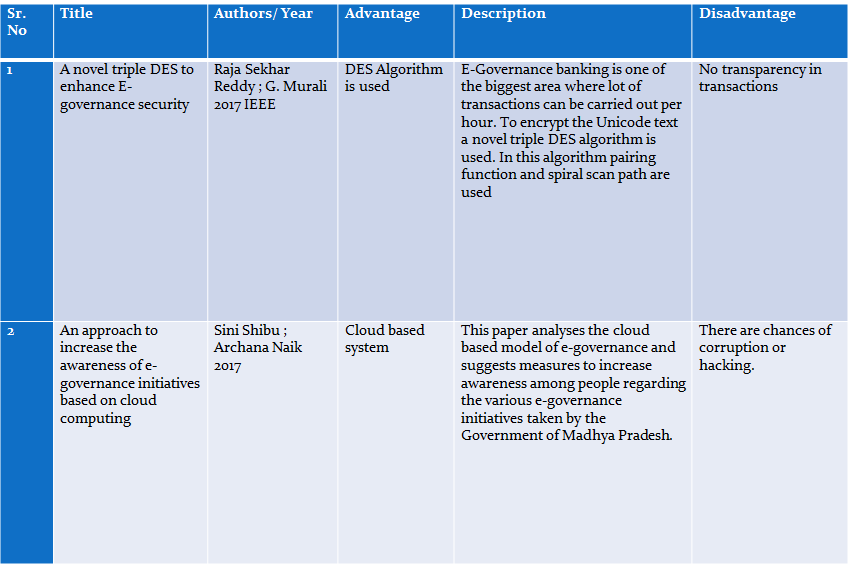
\includegraphics[scale=0.83	]{LS1}}
	    \caption{LITERATURE SURVEY TABLE 1}
	    \label{fig:LITERATURE SURVAY TABLE 1}
	\end{figure}
\end{center}
\newpage

\begin{center}
	\begin{figure}[!htbp]
		\centering
		\fbox{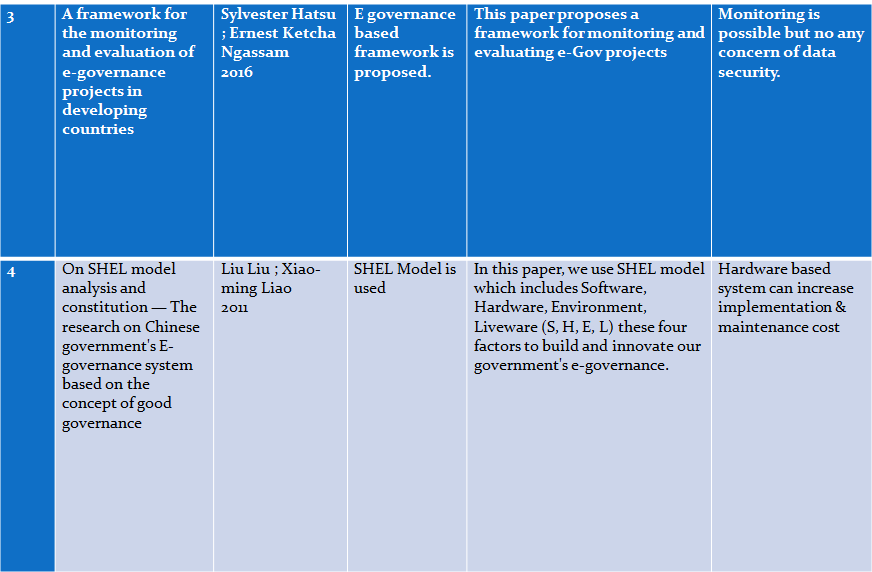
\includegraphics[scale=0.85	]{LS2}}
	    \caption{LITERATURE SURVEY TABLE 2}
	    \label{fig:LITERATURE SURVAY TABLE 2}
	\end{figure}
\end{center}
\newpage

\begin{center}
	\begin{figure}[!htbp]
		\centering
		\fbox{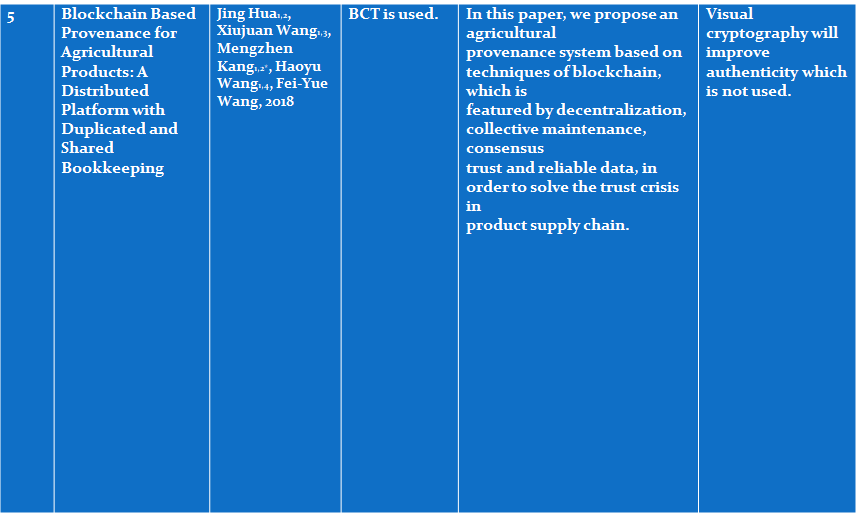
\includegraphics[scale=0.85	]{LS3}}
	    \caption{LITERATURE SURVEY TABLE 3}
	    \label{fig:LITERATURE SURVAY TABLE 3}
	\end{figure}
\end{center}
\newpage

\begin{center}
	\begin{figure}[!htbp]
		\centering
		\fbox{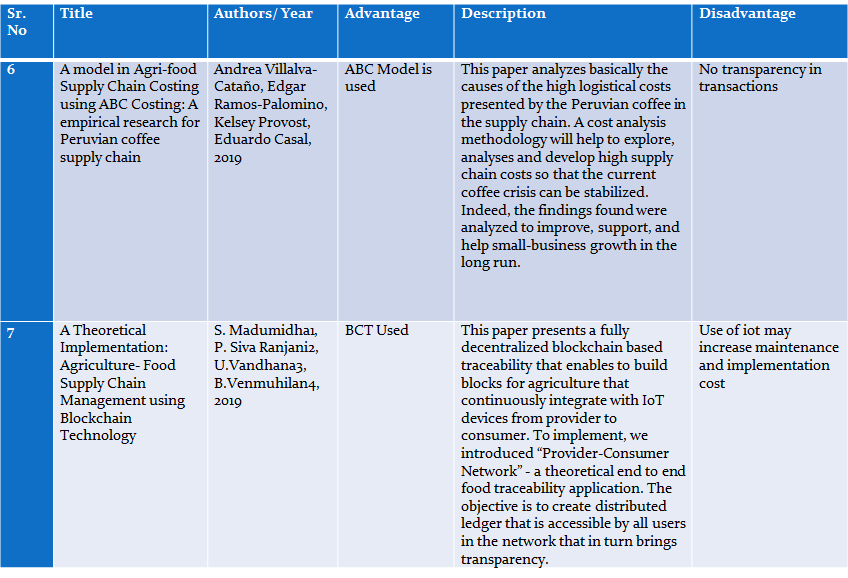
\includegraphics[scale=0.85	]{LS4}}
	    \caption{LITERATURE SURVEY TABLE 4}
	    \label{fig:LITERATURE SURVAY TABLE 4}
	\end{figure}
\end{center}
\newpage

\begin{center}
	\begin{figure}[!htbp]
		\centering
		\fbox{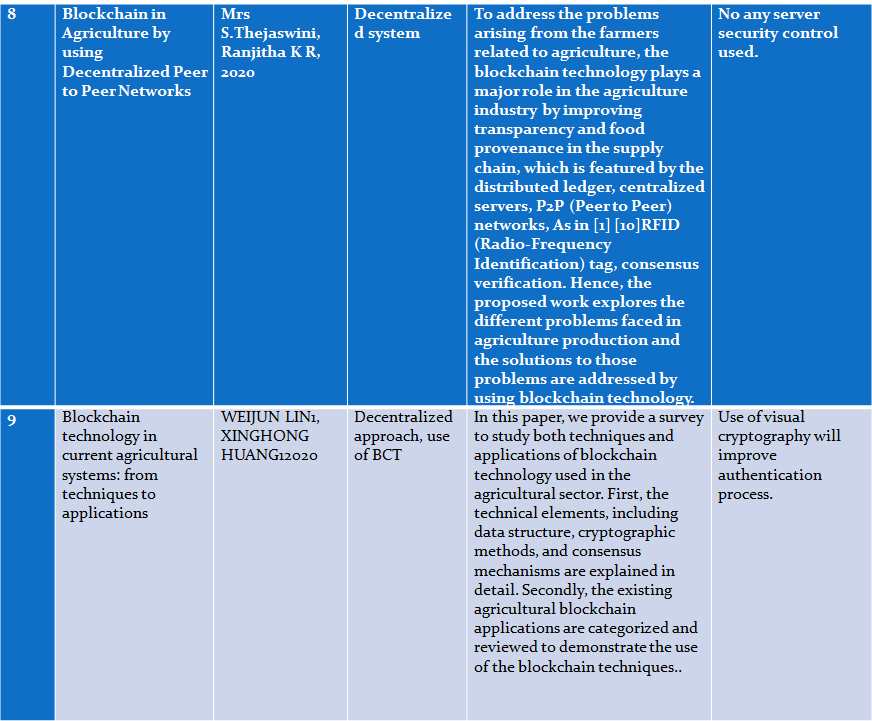
\includegraphics[scale=0.85	]{LS5}}
	    \caption{LITERATURE SURVEY TABLE 5}
	    \label{fig:LITERATURE SURVAY TABLE 5}
	\end{figure}
\end{center}
\newpage

\begin{center}
	\begin{figure}[!htbp]
		\centering
		\fbox{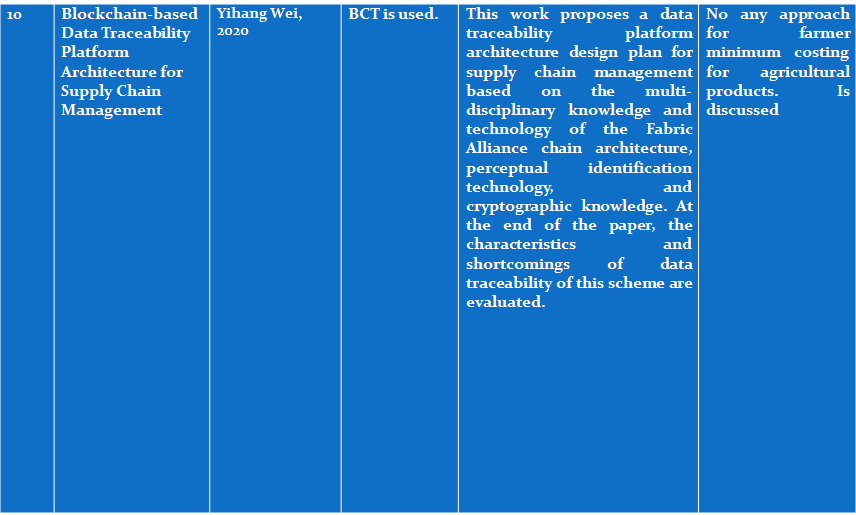
\includegraphics[scale=0.85	]{LS6}}
	    \caption{LITERATURE SURVEY TABLE 6}
	    \label{fig:LITERATURE SURVAY TABLE 6}
	\end{figure}
\end{center}
\newpage

\chapter{Software Requirement Specification}

%NNNNNNNNNNNNNNNNNNNNNNNNNNNNNNNNNNNNNNNNNNNNNNNNNNNNNNNNNNNNNNNNNNNNNNNNNNNNNNNNNNNNNNNNNNNNNNNNNNNNNNNNNNNNNNNNNNNNNN

\section{Project Scope}
\begin{itemize}
\item To develop prototype model for agricultural supply chain management.
\item This model will be run at local host using Glassfish server.
\item BCT features such as decentralization, cryptography and hash codes will be implemented.
\end{itemize}

\section{Assumptions and Dependencies}
\hspace*{0.5cm} This document will provide a general description of project, including user requirements, product perspective, and overview of requirements, general constraints. In addition, it will also provide the specific requirements and functionality needed for this project such as interface, functional requirements and performance requirements.

\subsection{User Classes and Characteristics}
\hspace*{0.5cm} Find the different user classes that you anticipate will use this product. User classes can be differentiated based on use frequency or product functions subset used or technical expertise or privilege levels or educational level and experience. It also describe the pertinent behavior or characteristics of each user class. Few requirements may limited only to specific user classes. Differentiate the very most important or useful user classes for this item or product from those who are less significant to satisfy.

\section{Functional Requirements}
\hspace*{0.5cm} Functional user requirements is nothing but very high-level statements about what the system should and also it should describe clearly an overview of  system services in detail.

\section{External Interface Requirements}
\subsection{User Interfaces}
\hspace*{0.5cm} The user interface or UI for the software should be compatible to be used by any standard browser such as IE, Mozilla or Google chrome. Using this UI user can have access to the system. The UI or user interface can be developed  by using many tool or software package like JFrame.

\subsection{Hardware Interfaces}
\hspace*{0.5cm} A hardware interface is needed to run the software. Java (JDK) and NetBeans compatible hardware is required which is minimal requirement. 

\subsection{Software Interfaces}
\hspace*{0.5cm} It uses Java as the front end programming tool. MySQL has been used as  back end application tool. Latest version of java anything higher than 7.0 can be used. 

\section{Non Functional Requirements}
\subsection{Performance Requirements}
\begin{itemize}
\item System can work optimal or faster on 4 GB or more of RAM.
\item The system is targeted to be available all time. Once there is a fatal error or system down, the system will provide understandable feedback to the user.
\end{itemize}

\subsection{Safety Requirements}
\begin{itemize}
\item  The system is designed in modules where errors can be detected.
\end{itemize}

\subsection{Security Requirements}
\begin{itemize}
\item The system is designed in modules where errors can be detected and fixed easily.
\end{itemize}

\subsection{Software Quality Attributes}
\begin{itemize}
\item \textbf{Usability: }\\
\hspace*{0.5cm} This relates to how easily people can use app/website. A measure of usability could be the time it takes for end users to become familiar with my app/website functions, without training or help.
\item \textbf{Reliability:}\\
\hspace*{0.5cm} This can be defined as the available time or UP time of software.
\item \textbf{Performance: }\\
\hspace*{0.5cm} This is essentially how fast app/website works. A performance requirement for the app/website could be start in less than 20 seconds.
\item \textbf{Security :}\\
\hspace*{0.5cm} Say that app/website saves all the previous code and lets you reuse a saved code.
\end{itemize}

\section{System Requirements}
\subsection{Database Requirements}
\textbf{MySQL Database}\\
\hspace*{0.5cm} MySQL is on open source database which is mainly a RDBMS i.e. relational database management system. As a database server, primary function of this software is to storing and retrieving data as requested by other from end software applications like java which may  Or may not run either on the same computer or on different computer. This can be across the network either in internet or intranet.

\subsection{Software Requirements}
\begin{enumerate}
\item \textbf{Operating System: } Microsoft Windows 7 and Above
\item \textbf{Programming Language: } Java
\item \textbf{IDE: } Netbeans
\end{enumerate}
\subsection{Hardware Requirements}
\begin{enumerate}
\item \textbf{Processor: } Intel Core I3 or Higher
\item \textbf{RAM: } 4 GB or Higher
\item \textbf{Hard Disk: } 100 GB (min)
\end{enumerate}

\section{Analysis Models: SDLC Model to be applied}
\textbf{SDLC model to be applied}\\
\textbf{Waterfall Model:}\\
\hspace*{0.5cm} The Waterfall Model is among very first and old model of software development life cycle. It is also called as a linear-sequential life cycle model. This is very simple in nature and easy to understand or use. This is step by step method so next step can only be begin once earlier has been completed. This is mainly used for small scale project. Constant or fixed requirement should be there for this type of model. 

\begin{center}
	\begin{figure}[!htbp]
		\centering
		\fbox{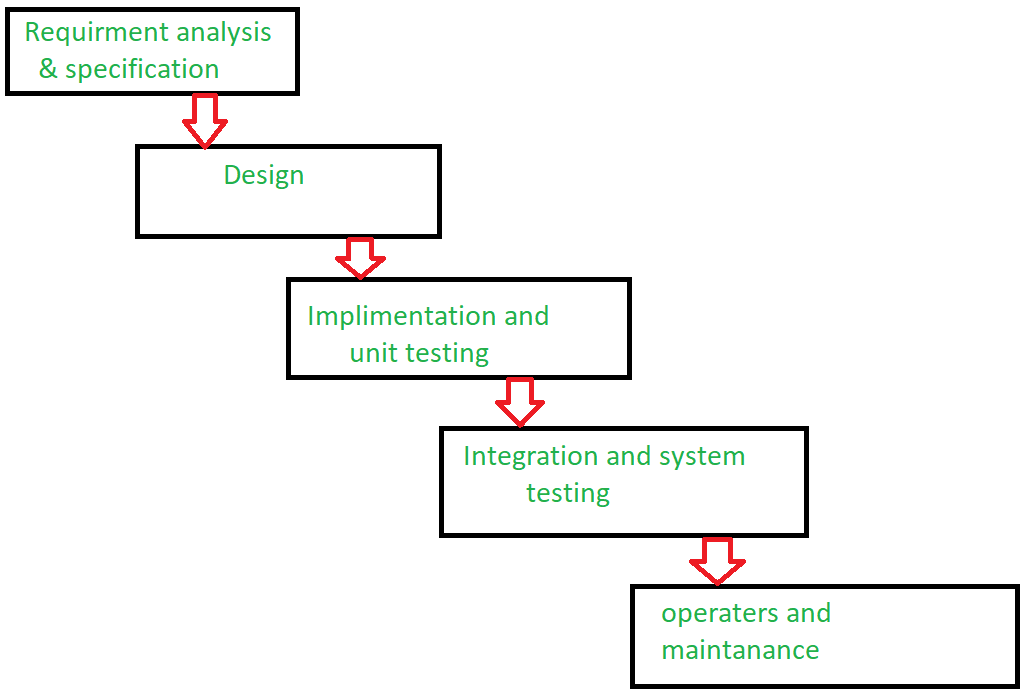
\includegraphics[scale=0.65	]{waterfall}}
	    \caption{Waterfall Model}
	    \label{fig:Waterfall Model}
	\end{figure}
\end{center}

%NNNNNNNNNNNNNNNNNNNNNNNNNNNNNNNNNNNNNNNNNNNNNNNNNNNNNNNNNNNNNNNNNNNNNNNNNNNNNNNNNNNNNNNNNNNNNNNNNNNNNNNNNNNNNNNNNNNNNN

\chapter{System Design}

%NNNNNNNNNNNNNNNNNNNNNNNNNNNNNNNNNNNNNNNNNNNNNNNNNNNNNNNNNNNNNNNNNNNNNNNNNNNNNNNNNNNNNNNNNNNNNNNNNNNNNNNNNNNNNNNNNNNNNN

\section{System Architecture}

\begin{center}
	\begin{figure}[!htbp]
		\centering
		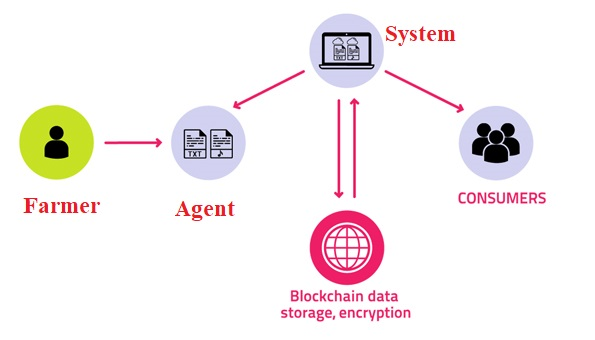
\includegraphics[scale=1.1]{architecture}
        \caption{System Architecture}
	    \label{fig:System Architecture}
	\end{figure}
\end{center}
Whenever any transaction will occur in the system , the record of that transaction is maintained in the form of hash value in a block. Each next block will get attached to the previous block and in this way a virtual block chain will occur. The hash value of a current block is generated using the data of a current block and the hash of the previous block. In this way if any of the block is tempered the subsequent all the block’s hash must be changed . Such multiple copies are maintained at different servers , which will assure the data security and confidentiality.  As everything is through application interface, it will maintain the transparency in the agricultural supply chain management.

\begin{center}
	\begin{figure}[!htbp]
		\centering
		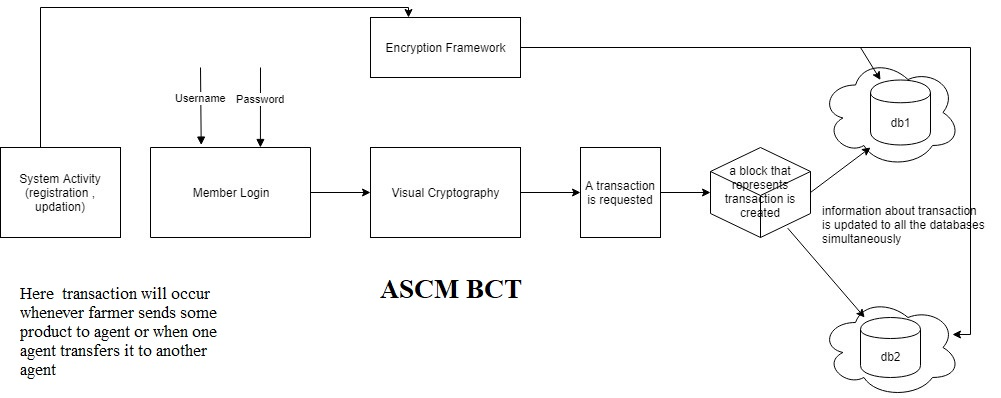
\includegraphics[scale=0.75]{architecture2}
        \caption{System Flow}
	    \label{fig:System Flow}
	\end{figure}
\end{center}
\newpage

\section{MATHEMATICAL MODEL}

Let
\newline
S be Closed system defined as, S = { Ip, Op, Ss, Su, Fi, A}

To select the input from the system and perform various actions from the set of actions A so that Su state can be attained.
\newline 
S={Ip,Op,Ss,Su,Fi,A}
\newline
Where,
\newline   
IP1={Username,Password, image}
\newline
Set of actions=A={F1,F2,F3,F4}
\newline
Where
\newline
F1= Send Mail
\newline
F2= Merge Images
\newline
F3= Encrypt Database
\newline
F4= Generate Hash
\newline
S=Set of users
\newline
Ss={rest state, registration state, login state}
\newline
Su- success state is successful analysis
\newline
Fi- failure state 
\newline
Objects:
\newline
1)	Input1: Ip1 = {Username, Password}
\newline
2)	Input2 : Ip2= {image from mail}
\newline
1)	Output1 : Op1 = Transaction Record 
\newline
2)	Output2 : Op2 = Encrypted Database
\newline
3)	Output3 : Op3 = Hash Codes.

\section{Data Flow Diagrams}
\hspace*{0.5cm} A data flow diagram (DFD) is a graphical representation of the ``flow" of data through an information system, modeling its process aspects. A DFD is often used as a preliminary step to create an overview of the system, which can later be elaborated. DFDs can also be used for the visualization of data processing.  

\subsection{Level 0 Data Flow Diagram}
\begin{center}
	\begin{figure}[!htbp]
		\centering
		\fbox{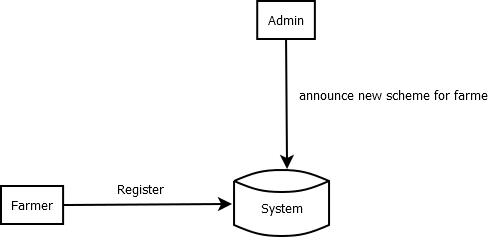
\includegraphics[scale=0.70]{dfd0}}
   	    \caption{Level 0 Data Flow Diagram}
	    \label{fig:Level 0 Data Flow Diagram}
	\end{figure}
\end{center}

\subsection{Level 1 Data Flow Diagram}
 \begin{center}
	\begin{figure}[!htbp]
		\centering
		\fbox{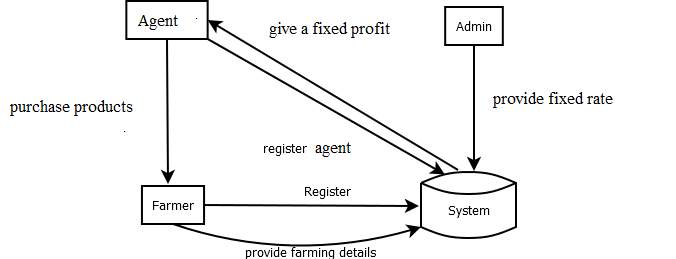
\includegraphics[scale=0.80]{dfd1}}
	    \caption{Level 1 Data Flow Diagram}
	    \label{fig:Level 1 Data Flow Diagram}
	\end{figure}
\end{center}

\newpage
\section{Entity Relationship Diagrams}
\hspace*{0.5cm} An entity relationship diagram (ERD) shows the relationships of entity sets stored in a database. An entity in this context is an object, a component of data. An entity set is a collection of similar entities. These entities can have attributes that define its properties. By defining the entities, their attributes, and showing the relationships between them, an ER diagram illustrates the logical structure of databases.

\begin{center}
	\begin{figure}[!htbp]
		\centering
		\fbox{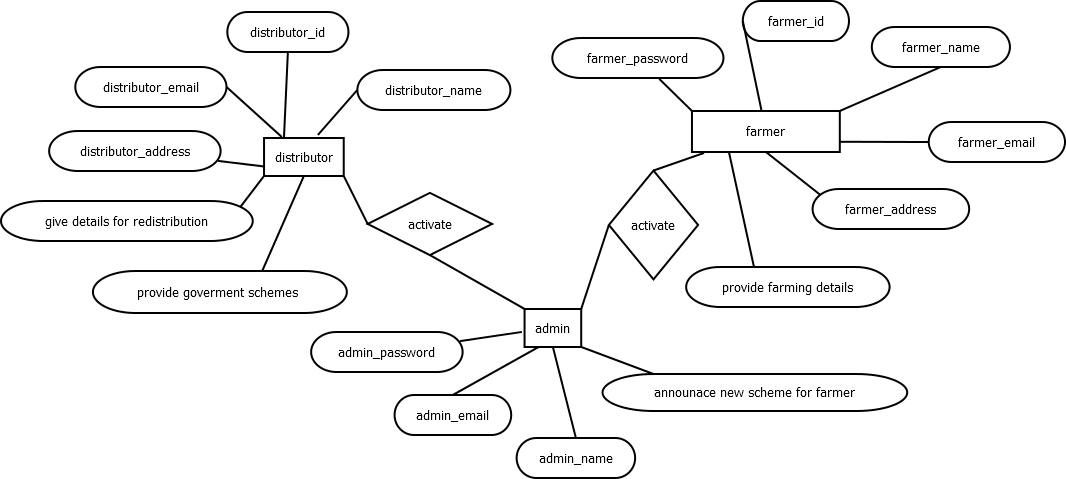
\includegraphics[scale=0.35]{er}}
  	    \caption{Entity Relationship Diagrams}
	    \label{fig:Entity Relationship Diagrams}
	\end{figure}
\end{center} 

\newpage
\section{UML Diagrams}
\subsection{Class Diagram}
\hspace*{0.5cm} A class diagram in the world of Unified Modeling Language or UML can be defined as a type of static structure diagram which mainly defines the structure of a system. It works by showing the system’s classes and their attributes and operations or methods also the relationships among objects.

\begin{center}
	\begin{figure}[!htbp]
		\centering
		\fbox{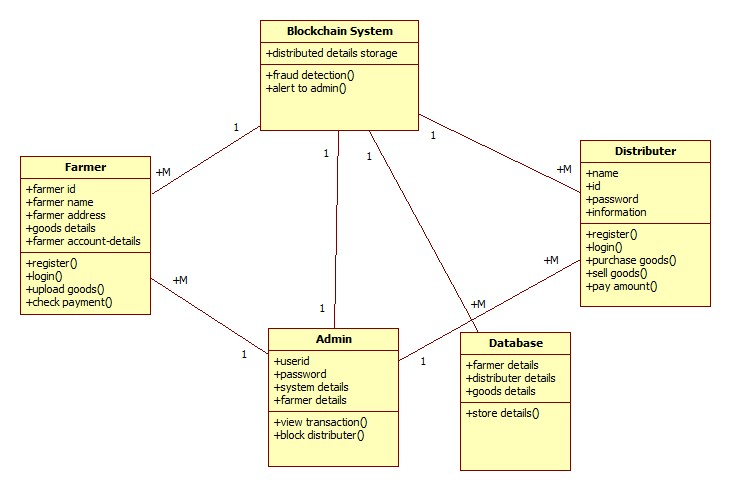
\includegraphics[scale=0.52]{class}}
  	    \caption{Class Diagram}
	    \label{fig:Class Diagram}
	\end{figure}
\end{center}

\newpage
\subsection{Use Case Diagram}
\hspace*{0.5cm} Dynamic behavior is most important aspect to capture the model of any system. Dynamic behavior can be defined as the behavior of the system when it is running or operating. Static behavior is not sufficient to model a system rather dynamic behavior is more important than static behavior.

\begin{center}
	\begin{figure}[!htbp]
		\centering
		\fbox{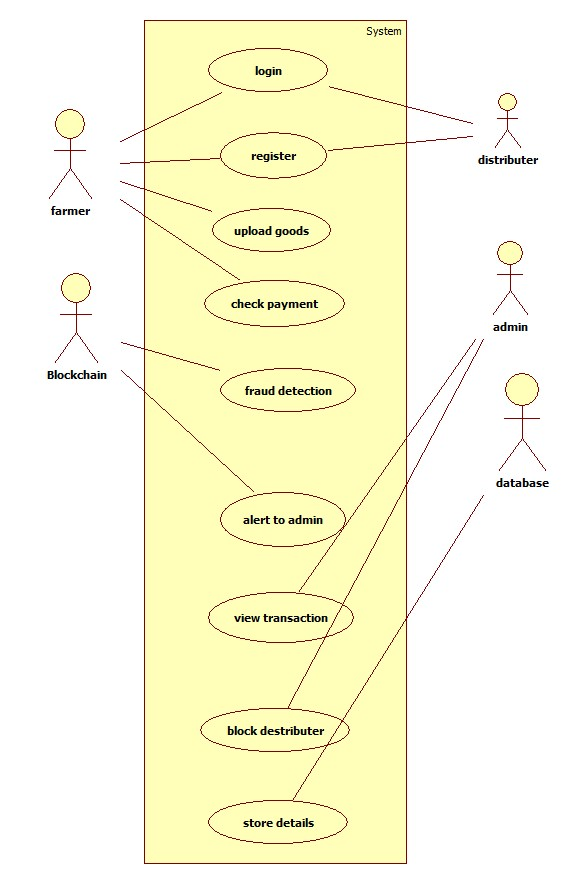
\includegraphics[scale=0.55]{usecase}}
	    \caption{Use Case Diagram}
	    \label{fig:Use Case Diagram}
	\end{figure}
\end{center}

\newpage
\subsection{Sequence Diagram}
\hspace*{0.5cm} Sequence diagrams can be used to provide a graphical representation of object  interactions or object coordination over the time. These basically displays a actor or user, and the objects and components they interact with in the execution of a use case. The sequence diagrams displays the own of messages from one object to another object, and as such correspond to the methods and events supported by a class/object.

\begin{center}
	\begin{figure}[!htbp]
		\centering
		\fbox{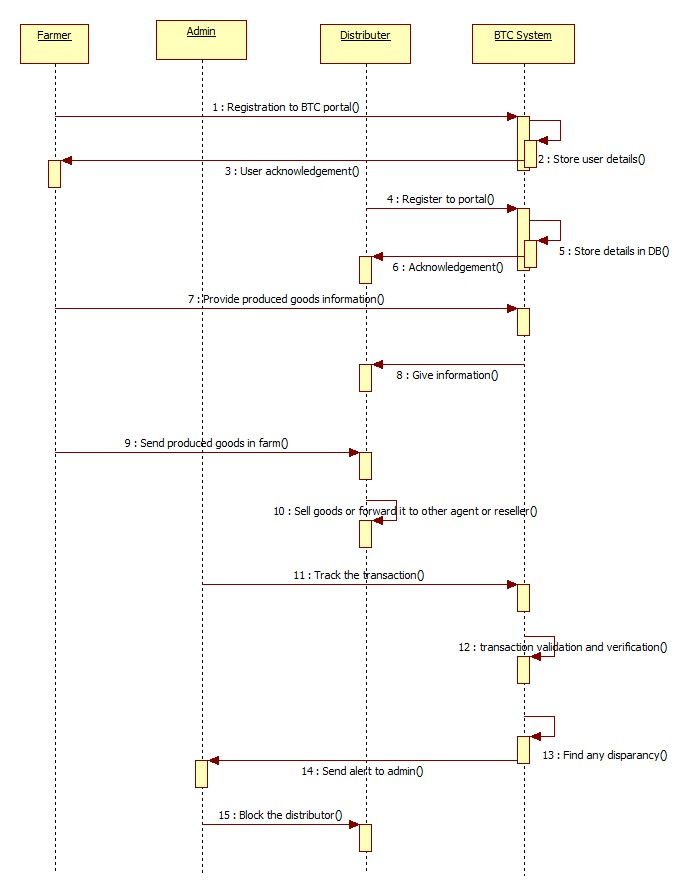
\includegraphics[scale=0.50]{sequence}}
 	    \caption{Sequence Diagram}
	    \label{fig:Sequence Diagram}
	\end{figure}
\end{center}

\newpage
\subsection{Activity Diagram}
\hspace*{0.5cm} Activity diagram can be defined as a flowchart to display the flow from one activity to another activity. These activities could be described as an operation of the system. The control flow usually is drawn from one operation of application to another. This can be branched or sequential, or concurrent also. Activity diagrams can deal with all or many type of flow control and used different elements such as join or fork.

\begin{center}
	\begin{figure}[!htbp]
		\centering
		\fbox{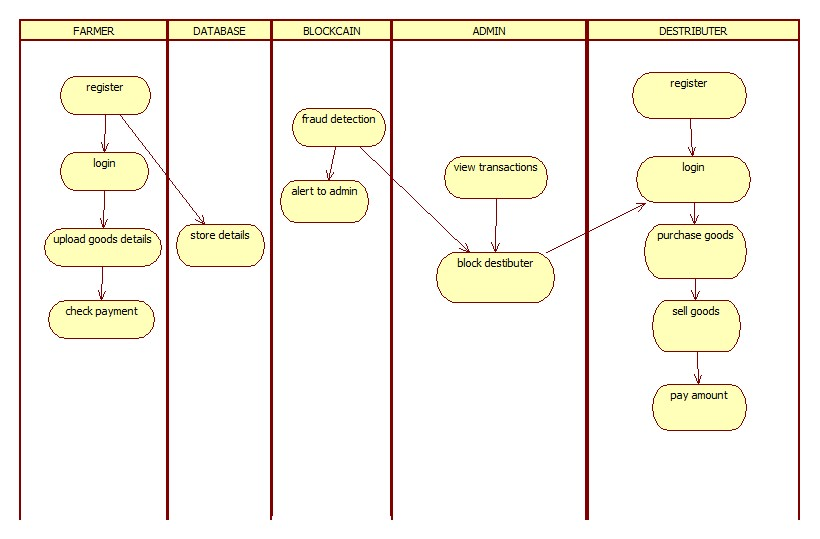
\includegraphics[scale=0.45]{activity}}
	    \caption{Activity Diagram}
	    \label{fig:Activity Diagram}
	\end{figure}
\end{center}
\chapter{PROJECT PLAN}
\def\arraystretch{1.3}
  \begin{tabular}{|c|c|p{9.2cm}|}
  \hline    
\textbf{Phase}	&\textbf{Task}	&\textbf{Description}	\\ \hline	   
Phase 1 &Analysis &Analyze the information related to Project Topic \\ \hline
Phase 2 & System Design &Assign the module and design the process flow Control \\ \hline
Phase 3 &Implementation &Implement the code for all the modules and integrate all the modules \\ \hline
Phase 4 &Testing &Test the code and overall process weather the process works
properly Test the code and over all process weather the process works properly \\ \hline
Phase 5 &Maintenance & Modification of a software product after delivery to improve performance or maintainability. \\ \hline
\end{tabular}



\subsection{Reconciled Estimates}
\section{Project Estimate}
{\renewcommand{\arraystretch}{2}%
	\begin{table}[!htbp]
   
				\begin{tabular}{ |p{1cm}|p{4cm}|p{6cm}|  }
 \hline
 Sr.No. & Milestone Name & Milestone Description\\ 
 \hline
 1. & Requirement Analysis & Complete specification of system \\ 
 \hline
2. & High level design & Identify the modules and the different  entities and their relationships\\
 \hline
 3. & Detailed design & GUI design, program specification etc \\ 
 \hline
4. & Build & Writing code for different modules\\
\hline
5.	& Testing  & Test the different modules together  \\
\hline
6. & Final Review and Deployment & Checking all the requirements are fulfilled \\
\hline
\end{tabular}
\caption{Project Estimate}
	\label{tab:hreq}
\end{table}
\subsection{COCOMO Model}
Cocomo (Constructive Cost Model) is a regression model based on LOC, i.e number of Lines of Code. It is a procedural cost estimate model for software projects and often used as a process of reliably predicting the various parameters associated with making a project such as size, effort, cost, time and quality. It was proposed by Barry Boehm in 1970 and is based on the study of 63 projects, which make it one of the best-documented models. The key parameters which define the quality of any software products, which are also an outcome of the Cocomo are primarily Effort \& Schedule:
\begin{itemize}
\item Effort: Amount of labor that will be required to complete a task. It is measured in person-months units.\
\item Schedule: Simply means the amount of time required for the completion of the job, which is, of course, proportional to the effort put. It is measured in the units of time such as weeks, months.\\
\end{itemize}
\
Different models of Cocomo have been proposed to predict the cost estimation at different levels, based on the amount of accuracy and correctness required. All of these models can be applied to a variety of projects, whose characteristics determine the value of constant to be used in subsequent calculations. These characteristics pertaining to different system types are mentioned below.\\

Boehm’s definition of organic, semidetached, and embedded systems:
\begin{enumerate}
\item Organic – A software project is said to be an organic type if the team size required is adequately small, the problem is well understood and has been solved in the past and also the team members have a nominal experience regarding the problem.\
\item Semi-detached – A software project is said to be a Semi-detached type if the vital characteristics such as team-size, experience, knowledge of the various programming environment lie in between that of organic and Embedded. The projects classified as Semi-Detached are comparatively less familiar and difficult to develop compared to the organic ones and require more experience and better guidance and creativity. Eg: Compilers or different Embedded Systems can be considered of Semi-Detached type.\
\item Embedded – A software project with requiring the highest level of complexity, creativity, and experience requirement fall under this category. Such software requires a larger team size than the other two models and also the developers need to be sufficiently experienced and creative to develop such complex models.\
\end{enumerate}

\ All the above system types utilize different values of the constants used in Effort Calculations. Types of Models: COCOMO consists of a hierarchy of three increasingly detailed and accurate forms. Any of the three forms can be adopted according to our requirements. These are types of COCOMO model:
\begin{enumerate}
\item Basic COCOMO Model
\ The first level, Basic COCOMO can be used for quick and slightly rough calculations of Software Costs. Its accuracy is somewhat restricted due to the absence of sufficient factor considerations.\\


The basic COCOMO model estimates the software development effort using only lines of code.\\

\begin{center} $ E=a(KLOC)^b $\\
\end{center}
newline Where,\\
 E is the efforts applied by person in months, a = 3.0 and b = 1.12 , then KLOC=2.25\\
 Hence Efforts = 3.0 (1.8)1.12,\\
 E = 5.79 Person-month\\
 E = 6 Person-month\\
 Total of 6 Person-Month are required to complete the project successfully.\\

\begin{center} $ D=cb(E)^d b$\\
\end{center}
Where,\\
 D = Development time in chronological months, cb = 2.5 and db = 0.35, and E =6 Person-Month\\
 Hence, Development Time= 2.5 (1.8)0.35\\
 D = 3.07 months\\
 The approximate duration of project is 3 months.\\

 P = E/D\\
 Where,\\
 P = Number of persons to accomplish project.\\
Hence, Number of Persons required completing the project\\
 P = 6/3\\
 P = 2 persons\\
 Therefore 2 persons are required to successfully complete the project on schedule.\\

\item Intermediate COCOMO Model
\ Intermediate COCOMO takes these Cost Drivers into account and Detailed COCOMO additionally accounts for the influence of individual project phases, i.e in case of Detailed it accounts for both these cost drivers and also calculations are performed phase wise henceforth producing a more accurate result. These two models are further discussed below.
\item Detailed COCOMO Model
\ In detailed cocomo, the whole software is divided into different modules and then apply COCOMO in different modules to estimate effort and then sum the effort.\
\end{enumerate}

 Project Cost-\\

The model followed is the Constructive Cost Model(COCOMO) for estimating the effort required in completing the project. Like all the estimation models, the COCOMO Model requires sizing information. This information can be specified in the form of:
\begin{itemize}
\item Object Point
\item Function Point
\item Lines of source Code (KLOC) for our project, This work uses the sizing information in the form Lines of Source Code.
\item Total lines of code for our project, KLOC =1.8K (approx.).
\item Cost of each person per month, Cp=Rs.11,000/- (Per person-month)\\
 So, $ C=3 \times Cp=3 \times 11000= 33,000- $
\end{itemize} 
Therefore, the cost pf project is 33,000+10000(cost of camera approx) = 43,000/- (approx).\\

\subsection{Reconciled Estimates}
The part of the project will be hardware, which need to implement in our system on besides, also need to estimates the cost of the application which are designing keeping in mind the following factor:
\begin{itemize}
\item	Its market demand, what it has got to offer to the customer
\item Its relevance in the current world.
\item The extent to which it can adhere to its objective of secured data transmission.
\end{itemize}

\subsection{Project Resources}
1.  Designer: To design system and perform requirement gathering.

2.Developer: To develop system and provide to tester for testing

\newpage
\section{Risk Management}:
\subsection*{Risk Identification}
For risks identification, review of scope document, requirements specifications and schedule is done. Answers to questionnaire revealed some risks. Each risk is cate- gorized as per the categories mentioned in [?].You can refereed following risk iden- tification questionnaire.

1.	Have top software and customer managers formally committed to support the project?
Answer : Yes

2.	Are end-users enthusiastically committed to the project and the system/product to be built?
Answer : Yes

3.	Are requirements fully understood by the software engineering team and its customers?
Answer : Yes

4.	Have customers been involved fully in the definition of requirements?
Answer : Yes

5.	Do end-users have realistic expectations?
Answer : Yes

6.	Does the software engineering team have the right mix of skills?
Answer : Yes

7.	Are project requirements stable?
Answer : Yes

8.	Is the number of people on the project team adequate to do the job?
Answer : Yes

9.	Do all customer/user constituencies agree on the importance of the project and on the requirements for the system/product to be built?
Answer : Yes

5.2.2	NP Hard

A problem is NP-hard if solving it in polynomial time would make it possible to solve all problems in class NP in polynomial time. Some NP-hard problems are also in NP (these are called ”NP-complete”), some are not. If you could reduce an NP problem to an NP-hard problem and then solve it in polynomial time, you could

solve all NP problems. Also, there are decision problems in NP-hard but are not NP-complete, such as the infamous halting problem

5.2.3	Risk Analysis

•	Technical Risk:
The probability of loss incurred through the execution of a technical process in which the outcome is uncertain. Untested engineering, technological or manufacturing procedures entail some level technical risk that can result in the loss of time, resources, and possibly harm to individuals and facilities. Like mobile phone battery off, network error in user and server, multiple requests at time.
•	Operational Risk:
Operational risk is the prospect of loss resulting from inadequate or failed procedures, systems or policies. Employee errors. Systems failures. Fraud or other criminal activity. Any event that disrupts business processes. Like user registration, login, send request to service provider.
\newline
\newline
•	Schedule Risk:
Schedule risk is the risk that the project takes longer than scheduled. It can lead to cost risks, as longer projects always cost more, and to performance risk, if the project is completed too late to perform its intended tasks fully.
\newline
\newline
•	Business Risk:
Business risk is the possibilities a company will have lower than anticipated profits or experience a loss rather than taking a profit. Business risk is influ- enced by numerous factors, including sales volume, per-unit price, input costs, competition, and the overall economic climate and government regulations.

\newpage
\section{Project Schedule}:
\subsection{Project task set}
Major Tasks in the Project stages are:
\newline

\def\arraystretch{1.5}
  \begin{tabular}{| p{3cm} | p{3cm} |p{3cm}|}
\hline
\textbf{Priority (High to low)}	&\textbf{Risks}	&\textbf{Back-up plan}	 \\ \hline  
1	&Schedule	&Overtime	    \\ \hline 
2	&Operational	&Validation	   \\ \hline  
3	&Business	&Marketing	    \\ \hline 
4	&Technical	&-	  \\ \hline 
\end{tabular}
\newline\newline\newline
•	Task 1: Requirement Gathering\newline
•	Task 2: Literature Survey\newline
•	Task 3: System Design\newline
•	Task 4: Functionality Implementation\newline
•	Task 5: Testing
\subsection{Timeline Chart}
\begin{center}
	\begin{figure}[!htbp]
	
	\fbox{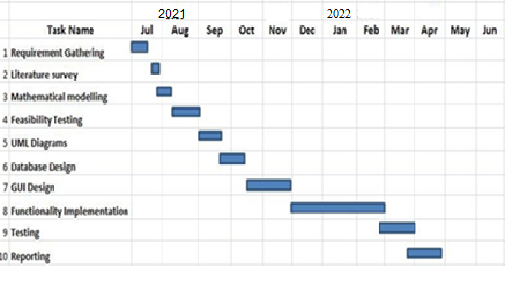
\includegraphics[width=15cm, height=10cm]{plan1}}
		  \caption{Timeline Chart}
	 
	\end{figure}
\end{center} 
\section{Team Organization}
\subsection{Team Structure}
Whatever activities are done related to the project that we all showing all details log to our guide. All the reporting are noted to the guide.

\begin{table}[!htbp]
\begin{center}
\def\arraystretch{1.5}
  \begin{tabular}{| c | p{6cm} | c |}
\hline
\textbf{Work Task}	&\textbf{Description}	&\textbf{Duration} \\ \hline
Literature Search	&Related  work  done  for  conceptual  data similarity	&6 weeks \\ \hline
System analysis	&Critical analysis and comparison of technologies  studied  and  results  achieved  in research	&4 weeks \\ \hline
Design and Planning	&Modeling and design and dataset searching or creation	&8 weeks \\ \hline
Implementation	&Divided into phases	& \\ \hline
Phase A	&Implementation module 1	&2 weeks \\ \hline
Phase B	&Implementation module 2	&2 weeks \\ \hline
Phase C	&Implementation module 3	&2 weeks \\ \hline
System Testing	&Test system quality, fix errors if any and improve if needed. Test system for different data sets	&3 weeks \\ \hline
Final Report	&Prepare and upload Initial Report	&2 weeks \\ \hline
Initial Report	&Prepare and upload Initial Report	&2 weeks \\ \hline
\end{tabular}
 \caption {Time line Chart}
 \label{tab:Timeline Chart}
\end{center}
\end{table}
\newpage
\chapter{Project Implementation}
\section{Overview of Project Modules}
BCT: First and foremost, blockchain is a public electronic ledger built around a P2P system that can be openly shared among disparate users to create an unchangeable record of transactions, each time-stamped and linked to the previous one. Every time a set of transactions is added, that data becomes another block in the chain (hence, the name). Blockchain can only be updated by consensus between participants in the system, and once new data is entered it can never be erased. It is a write-once, append-many technology, making it a verifiable and auditable record of each and every transaction.
Famer will transfer the products to the agent through the application interface, agent in turn will transfer any product to another agent through application interface only. Also the record of each and every transaction will be maintained at different places which will maintain transparency also the database is secured through AES. System login is secured through visual cryptography.
\section{Tools and Technologies Used:}
JDK 1.8 Installation
1.	Double click jdk-8-ea-bin-b32-windows-i586 to run the installation program.
JDK License dialog displayed. Accept the license in order to install JDK.

2.	The JRE Custom setup dialog enables you to choose a custom directory for JRE Files.
3.	The complete dialog indicates a successful installation.

Net Beans IDE 7.3.1 Installation
To install the software:

1.	After the download completes, run the installer. For Windows, the installer executable file has the .exe extension. Double-click the installer file to run it.
2.	If you downloaded the All bundle, you can customize your installation. Per- form the following steps at the Welcome page of the installation wizard:
a.	Click Customize.
b.	In the Customize Installation dialog box, make your selections.

•	At the Welcome page of the installation wizard, click Next. At the License agreement page, review the license agreement, click the acceptance check box, and click Next. At the JUnit License Agreement page, decide if you want to install JUnit and click the appropriate option, click Next. At the NetBeans IDE installation page, do the following:
•	Accept the default installation directory for the NetBeans IDE or specify an- other directory. Note: The installation directory must be empty and the user profile you are using to run the installer must have read/ write permissions for this directory.
•	Accept the default JDK installation to use with the NetBeans IDE or select   a different installation from the drop-down list. If the installation wizard did not find a compatible JDK installation to use with the Net-Beans IDE, your JDK is not installed in the default location. In this case, specify the path to an installed JDK and click Next, or cancel the current installation. After installing the required JDK version you can restart the installation.

•	If you are installing Apache Tomcat, on its installation page, accept the default installation directory or specify another installation location. Click Next.
•	At the Summary page, verify that the list of components to be installed is correct and that you have adequate space on your system for the installation.
•	Click Install to begin the installation.
•	At the Setup Complete page, provide anonymous usage data if desired, and click Finish.

MySQL Database

Microsoft SQL Server is a relational database management system developed by Mi- crosoft. As a database server, it is a software product with the primary function of storing and retrieving data as requested by other software applications which may run either on the same computer or on another computer across a network (includ- ing the Internet). Microsoft markets at least a dozen different editions of Microsoft SQL Server, aimed at different audiences and for workloads ranging from small single-machine applications to large Internet-facing applications with many concur- rent users.
\section{Algorithm Details:}
Algorithm:

6.3.1. AES is used to encrypt the database.\newline
The encryption process uses a set of specially derived keys called round keys. 
These are applied, along with other operations, on an array of data that holds exactly one block of data, the data to be encrypted. 
This array we call the state array.\newline


STEPS:\newline

\begin{itemize}


\item Derive the set of round keys from the cipher key.\newline
\item Initialize the state array with the block data (plaintext).\newline
\item Add the initial round key to the starting state array.\newline
\item Perform nine rounds of state manipulation.\newline
\item Perform the tenth and final round of state manipulation\newline
\item Copy the final state array out as the encrypted data (ciphertext).\newline
\end{itemize}

6.3.2.  SHA 256:Hash Function\newline

SHA-256 (secure hash algorithm, FIPS 182-2) is a cryptographic hash function with digest length of 256 bits. It is a keyless hash function; that is, an MDC (Manipulation Detection Code). A message is processed by blocks of 512 = 16 × 32 bits, each block requiring 64 rounds
A cryptographic hash (sometimes called ‘digest’) is a kind of ‘signature’ for a text or a data file. SHA-256 generates an almost-unique 256-bit (32-byte) signature for a text.A hash is not ‘encryption’ – it cannot be decrypted back to the original text (it is a ‘one-way’ cryptographic function, and is a fixed size for any size of source text). 
This makes it suitable when it is appropriate to compare ‘hashed’ versions of texts, as opposed to decrypting the text to obtain the original version.

\begin{center}
	\begin{figure}[!htbp]
		\centering
		\fbox{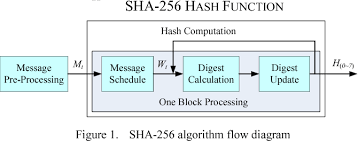
\includegraphics[scale=1.5]{SHA256}}
	    \caption{SHA 256 Diagram}
	    \label{fig:SHA 256 Diagram}
	\end{figure}
\end{center}


\chapter{Software Testing}
\section{Types of Testing}
\subsection{Unit Testing}
Unit testing is the testing of an individual unit or group of related units. It falls under the class of white box testing. It is often done by the programmer to test that the unit he/she has implemented is producing expected output against given input.
\subsection{Alpha Testing}
It is the most common type of testing used in the Software industry. The objective of this testing is to identify all possible issues or defects before releasing it into   the market or to the user. Alpha testing is carried out at the end of the software development phase but before the Beta Testing. Still, minor design changes may be made as a result of such testing. Alpha testing is conducted at the developer’s site. In-house virtual user environment can be created for this type of testing.
\subsection{Acceptance Testing}
An acceptance test is performed by the client and verifies whether the end to end the flow of the system is as per the business requirements or not and if it is as per the needs of the end user. Client accepts the software only when all the features and functionalities work as expected. It is the last phase of the testing, after which the software goes into production. This is also called User Acceptance Testing (UAT).
\subsection{Beta Testing}
Beta Testing is a formal type of software testing which is carried out by the customer. It is performed in the Real Environment before releasing the product to the market for the actual end users. Beta testing is carried out to ensure that there are no major failures in the software or product and it satisfies the business requirements from an end-user perspective. Beta testing is successful when the customer accepts the software. Usually, this testing is typically done by end-users or others. It is the  final testing done before releasing an application for commercial purpose. Usually, the Beta version of the software or product released is limited to a certain number of users in a specific area. So end user actually uses the software and shares the feedback to the company. Company then takes necessary action before releasing the software to the worldwide.
\subsection{Performance Testing}
This term is often used interchangeably with ‘stress’ and ‘load’ testing. Performance Testing is done to check whether the system meets the performance requirements. Different performance and load tools are used to do this testing.
\subsection{Security Testing}
It is a type of testing performed by a special team of testers. A system can be pen- etrated by any hacking way. Security Testing is done to check how the software or application or website is secure from internal and external threats. This testing in- cludes how much software is secure from the malicious program, viruses and how secure and strong the authorization and authentication processes are. It also checks how software behaves for any hackers attack and malicious programs and how soft- ware is maintained for data security after such a hacker attack.
\subsection{White Box Testing}
White Box testing is based on the knowledge about the internal logic of an appli- cation’s code. It is also known as Glass box Testing. Internal software and code working should be known for performing this type of testing. Under these tests are based on the coverage of code statements, branches, paths, conditions etc.

\subsection{Black Box Testing}
Black Box testing also known as Behavioral testing, is a software testing method  in which the internal structure or design or implementation of the item being tested is not known to the tester. These test can be functional or non-functional, through usually functional. This method is named as so because the software program, in the eyes of the tester, is like a black box, inside which one cannot see. This method attempts to find error like incorrect or missing functions, interface error, behavior or performance error etc.
\subsection{Regression Testing}
Testing an application as a whole for the modification in any module or functionality is termed as Regression Testing. It is difficult to cover all the system in Regression Testing, so typically automation testing tools are used for these types of testing.
\subsection{System Testing}
Under System Testing technique, the entire system is tested as per the requirements. It is a Black-box type testing that is based on overall requirement specifications and covers all the combined parts of a system.
\subsection{Smoke Testing}
Whenever a new build is provided by the development team then the software testing team validates the build and ensures that no major issue exists. The testing team ensures that the build is stable and a detailed level of testing is carried out further. Smoke Testing checks that no show stopper defect exists in the build which will prevent the testing team to test the application in detail. If testers find that the major critical functionality is broken down at the initial stage itself then testing team can reject the build and inform accordingly to the development team. Smoke Testing is carried out to a detailed level of any functional or regression testing.
\subsection{Integration Testing}
Integration testing is testing in which a group of components are combined to pro- duce output. Also, the interaction between software and hardware is tested in inte- gration testing if software and hardware components have any relation. It may fall under both white box testing and black box testing. It has two testing under it. These are- (a) Top to bottom. (b) Bottom to top.
(a)	Top to bottom:In this, the system is divided into different modules. Each and every module is tested from top to bottom.
(b)	Bottom to top: In this type of testing, every module is tested individually and at the end all modules are integrated.

\section{Test Cases}:
\begin{table}[!htbp]
	\begin{center}
		\def\arraystretch{1.5}
		\begin{tabular}{| p{0.5cm} | p{1.5cm} |p{2.5cm}| p{2.5cm} | p{2.5cm} | p{1cm}| }
			\hline
			\textbf{No.} &	\textbf{Test Case}	& \textbf{User Input}& \textbf{Expected Result}	& \textbf{Actual Result} &	\textbf{Status} \\ \hline
			1.&	Register User&	User gives all the
			credentials asked
			by the system&	Registration successful&	Registration successful&	Pass\\ \hline
			1.&	Register User&	If User miss any
			information to
			enter&	Registration
			Failed&	Registration
			Unsuccessful please
			Try again&	Pass\\ \hline
			2.&	Login&	System takes the
			username and password&	Login successful&	Successful&	Pass\\ \hline
			2.&	Login&	If incorrect information is entered&	Login failed&	Login failed, please give correct password
			or username&	Pass\\ \hline
			3.&	Browse
			Image&	Click on browse
			Button&	Unless image is
			selected button
			should remain
			disabled&	Button is disabled
			Unless proper image
			is selected&	Pass\\ \hline
			4.&	Browse
			Button&	Click on browse
			Button&	Browse File Dialog should open&	Browse file dialog opened successfully&	Pass\\ \hline
			5.&	Select non
			image file&	Select image&	Error message to be shown&	Error messaged
			Is seen&	Pass\\ \hline
		\end{tabular}
		\caption {Test Cases}
		\label{tab:Test Cases}
	\end{center}
\end{table}

\chapter{Results}:

\section{Outcome}:

Transparent supply chain due to use of BCT, block chain of every transaction is maintained and can be tracked in future. 

\section{Screenshots}

\begin{center}
	\begin{figure}[!htbp]
		\centering
		\fbox{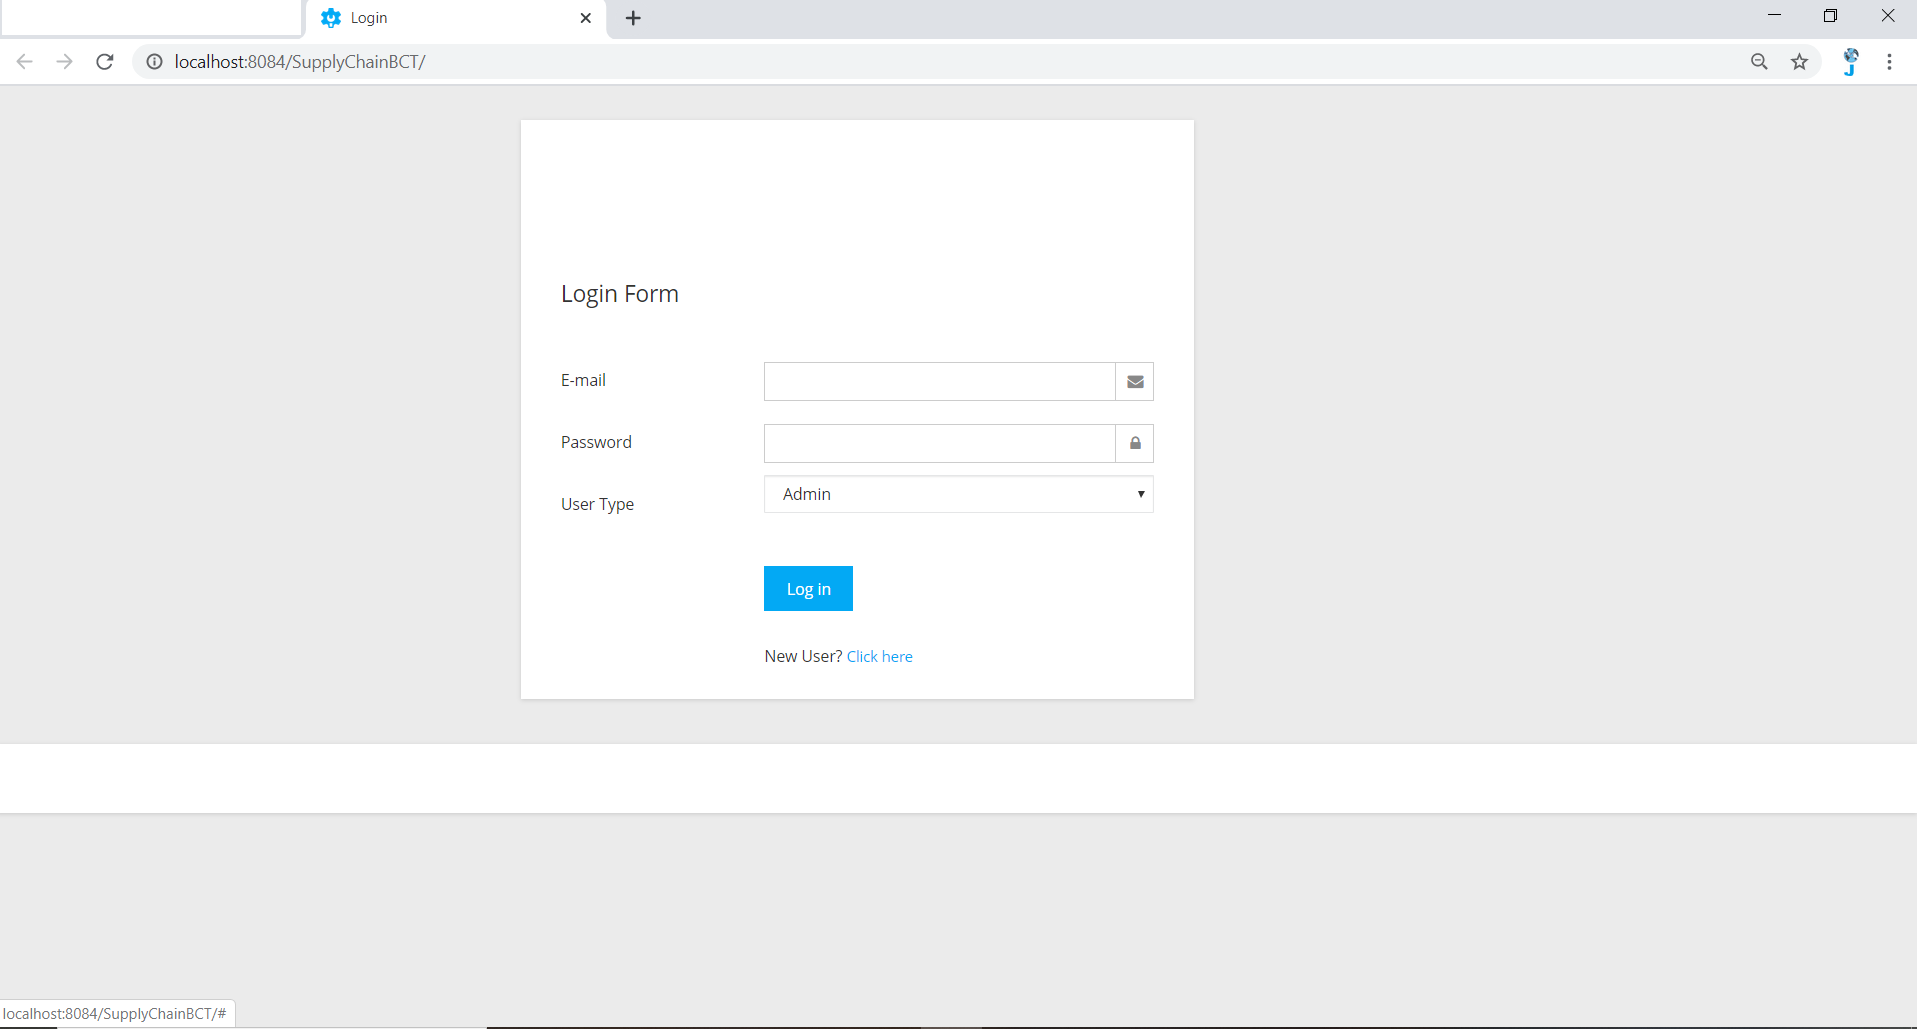
\includegraphics[scale=0.30]{1}}
		\caption{Login Page}
		\label{fig:Login}
	\end{figure}
\end{center}

\begin{center}
	\begin{figure}[!htbp]
		\centering
		\fbox{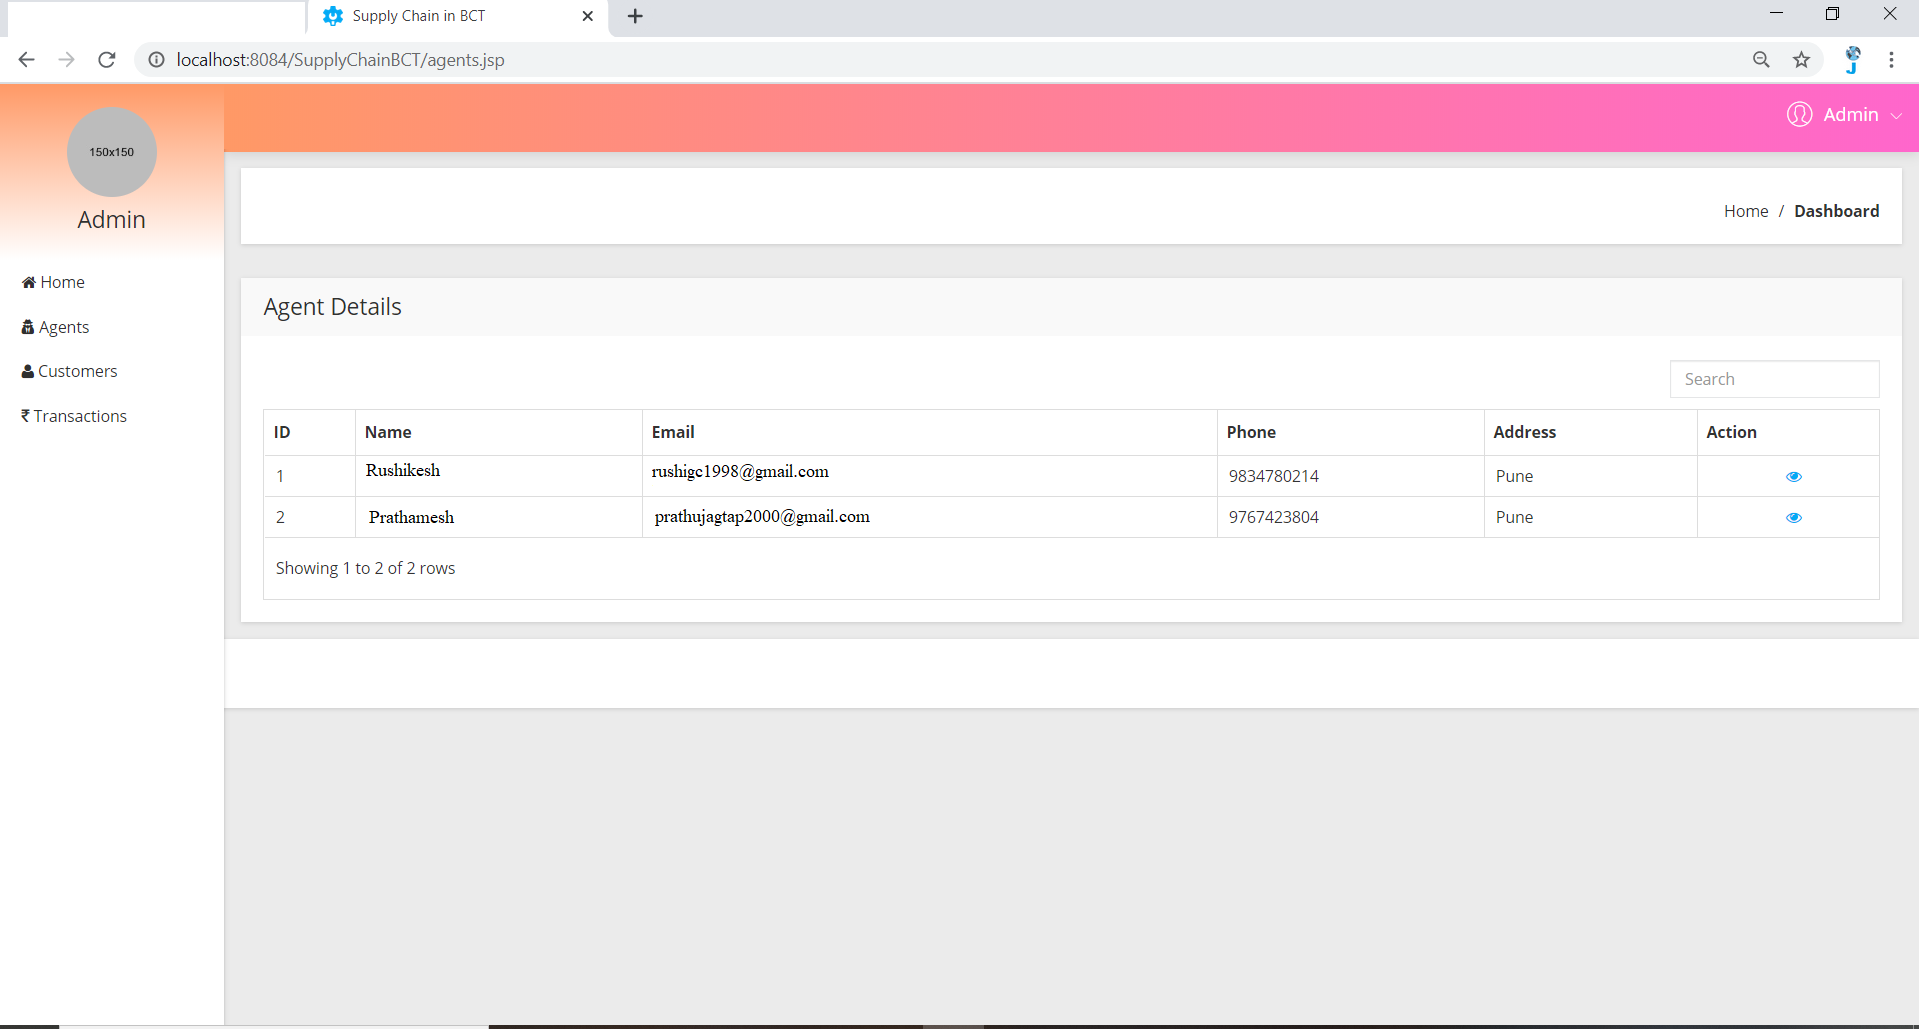
\includegraphics[scale=0.30]{2AdminViewAgents}}
		\caption{Admin View Agents}
		\label{fig:Admin View Agents}
	\end{figure}
\end{center}
\newpage

\begin{center}
	\begin{figure}[!htbp]
		\centering
		\fbox{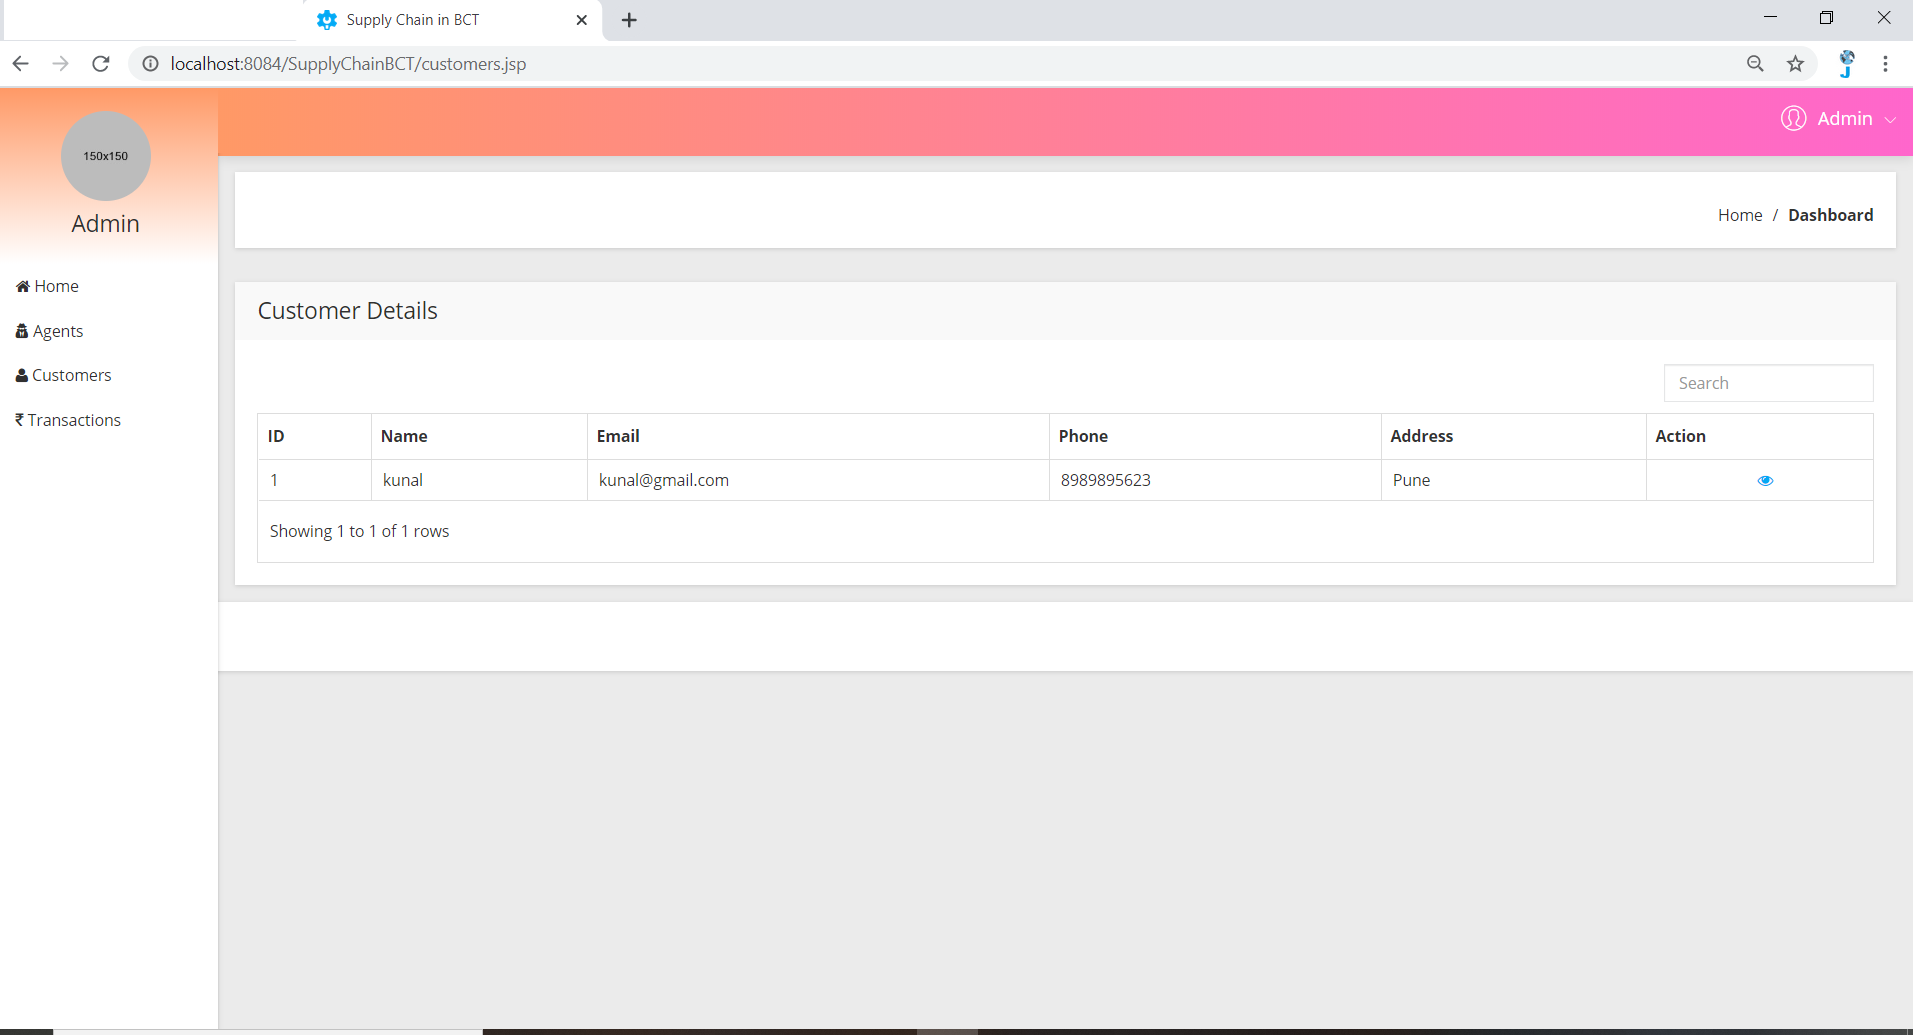
\includegraphics[scale=0.30]{3AdminViewCostumers}}
		\caption{Admin View Costumers}
		\label{fig:Admin View Costumers}
	\end{figure}
\end{center}

\begin{center}
	\begin{figure}[!htbp]
		\centering
		\fbox{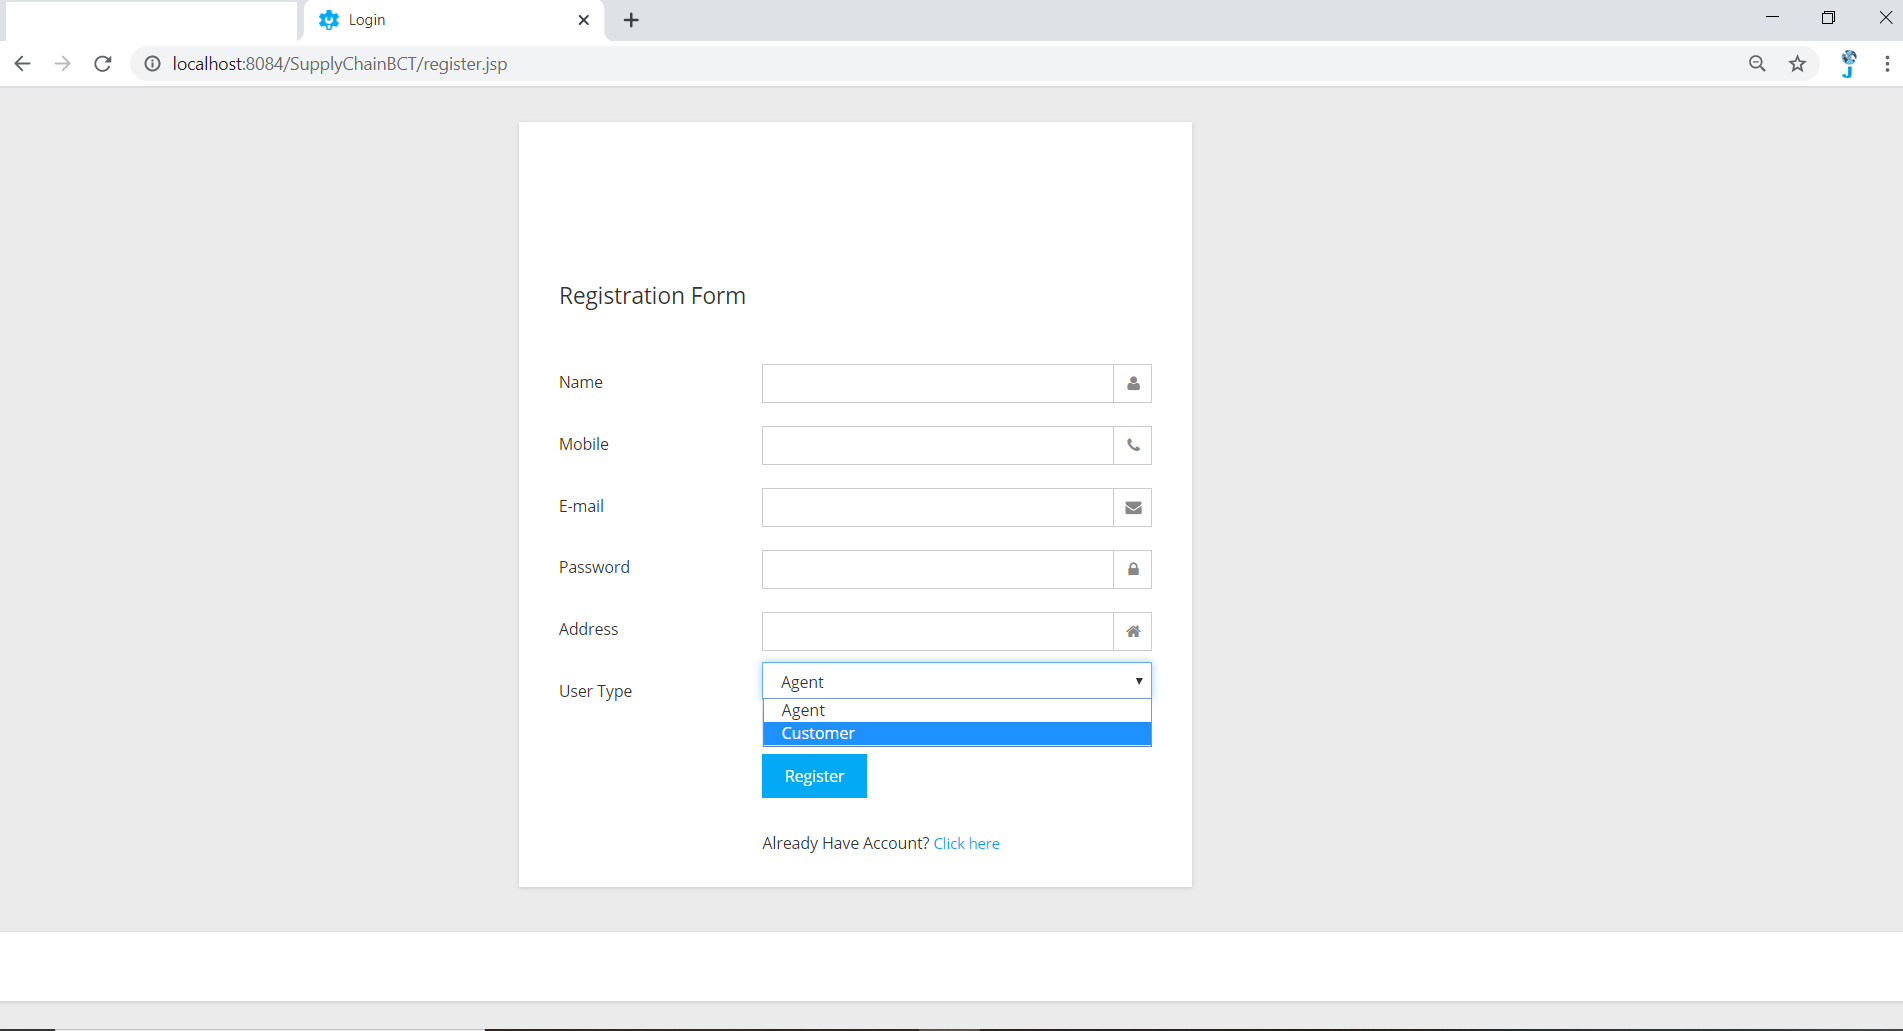
\includegraphics[scale=0.30]{4Registration}}
		\caption{User Registration}
		\label{fig:Registration}
	\end{figure}
\end{center}
\newpage

\begin{center}
	\begin{figure}[!htbp]
		\centering
		\fbox{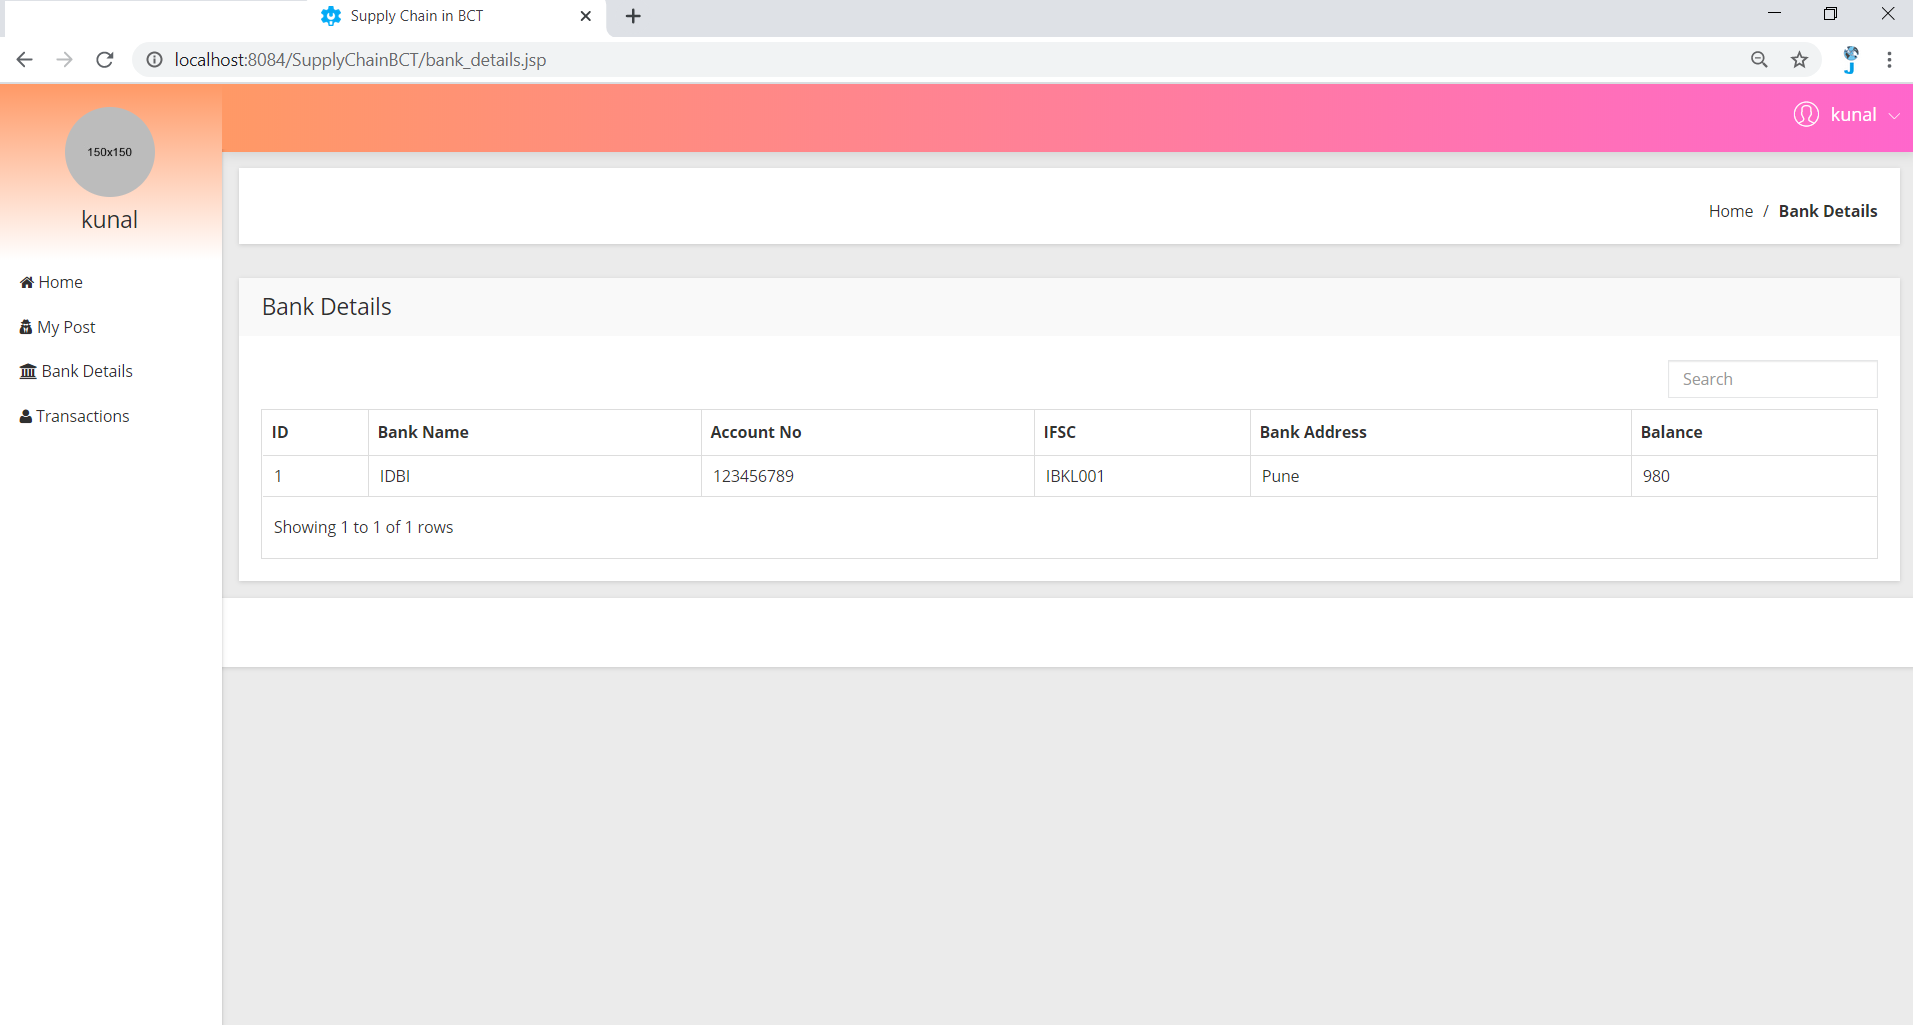
\includegraphics[scale=0.30]{5CostumerBankDetails}}
		\caption{Costumer Bank Details}
		\label{fig:Costumer Bank Details}
	\end{figure}
\end{center}

\begin{center}
	\begin{figure}[!htbp]
		\centering
		\fbox{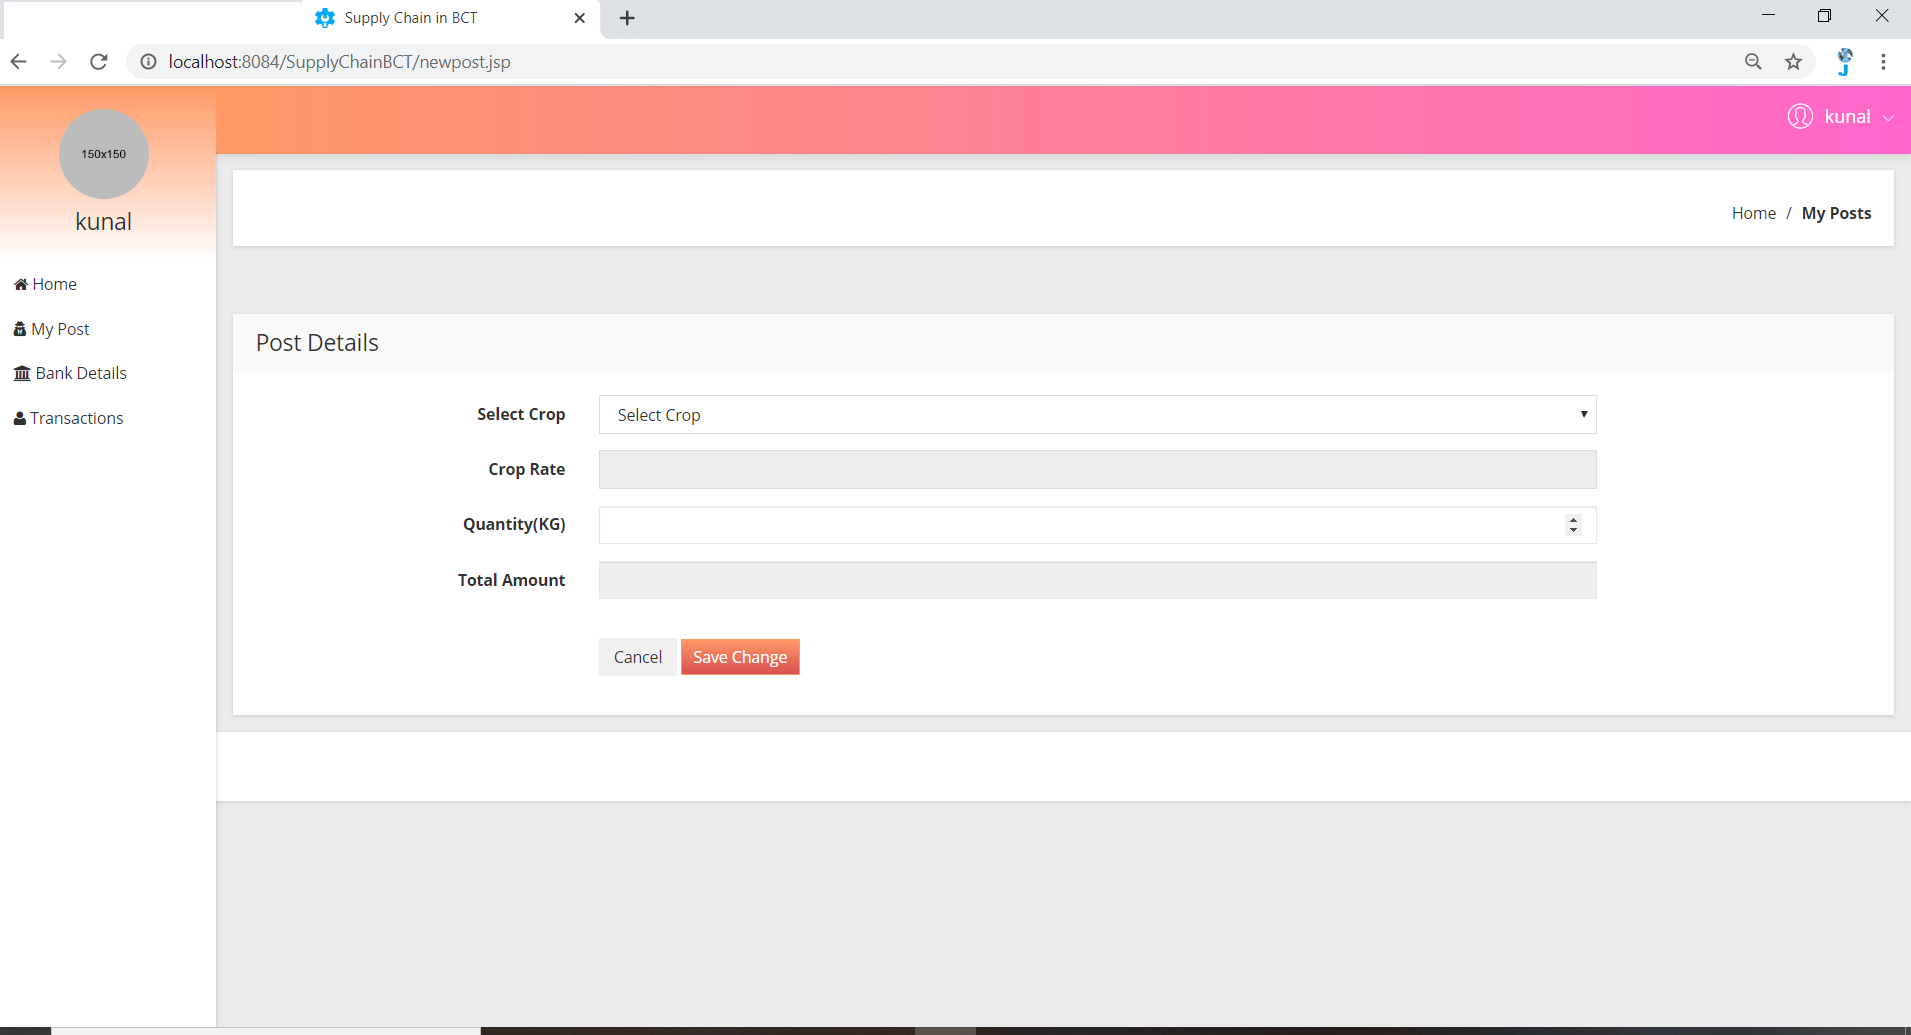
\includegraphics[scale=0.30]{6FarmerAddPost}}
		\caption{Farmer Add Post}
		\label{fig:Farmer Add Post}
	\end{figure}
\end{center}
\newpage

\begin{center}
	\begin{figure}[!htbp]
		\centering
		\fbox{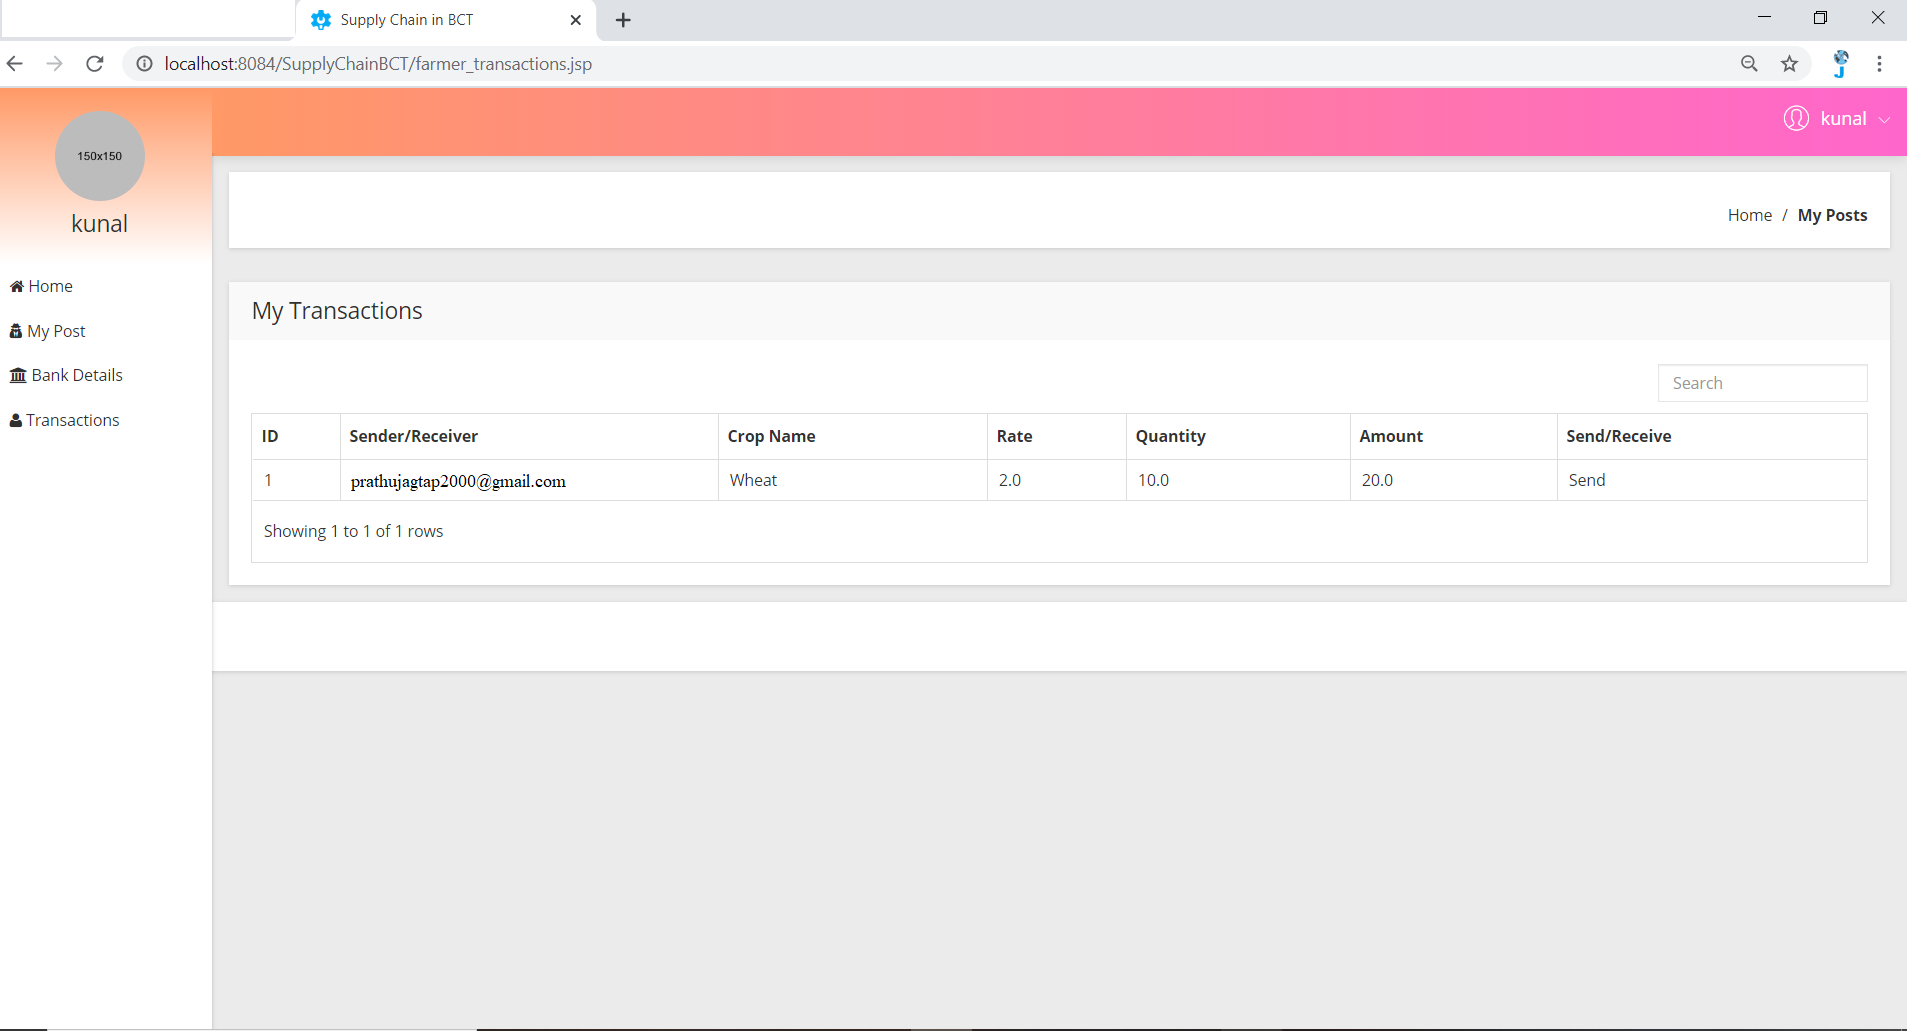
\includegraphics[scale=0.30]{8FarmerTransaction}}
		\caption{Farmer Transaction}
		\label{fig:Farmer Transaction}
	\end{figure}
\end{center}

\begin{center}
	\begin{figure}[!htbp]
		\centering
		\fbox{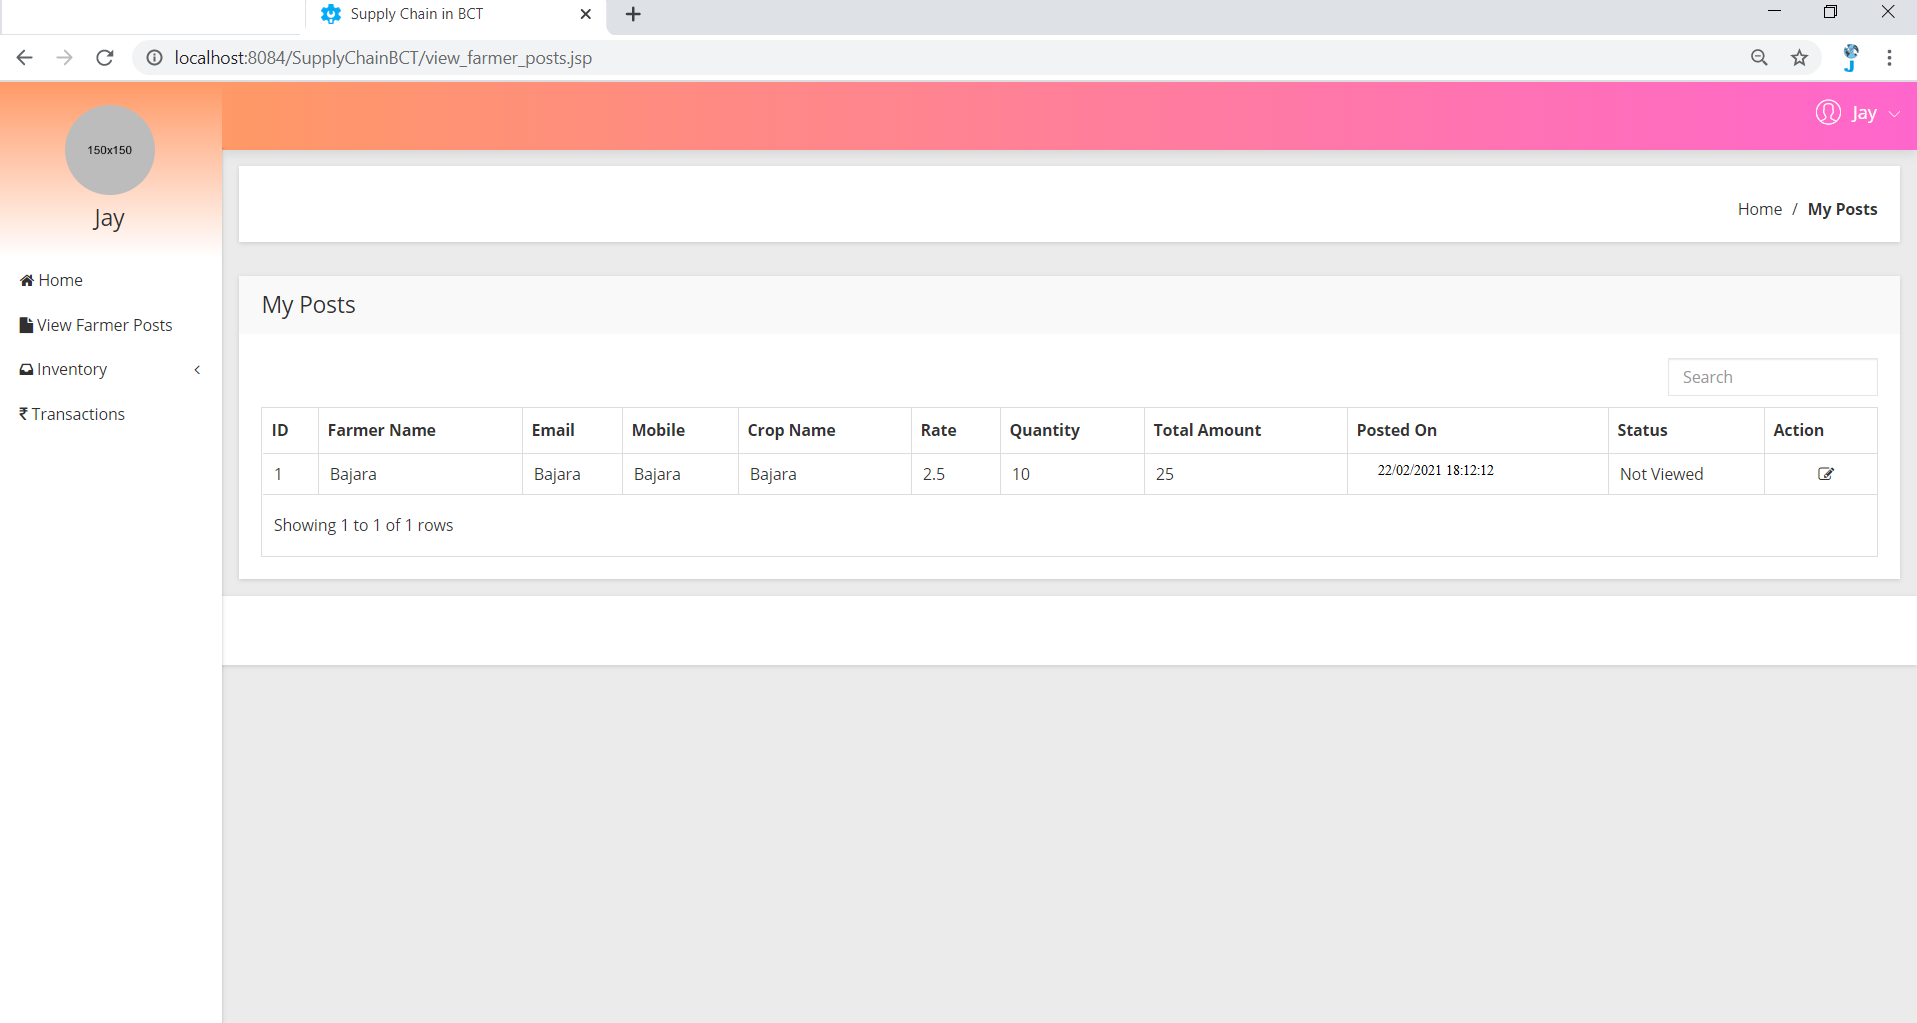
\includegraphics[scale=0.30]{9AgentViewFarmerPost}}
		\caption{Agent View Farmer Post}
		\label{fig:Agent View Farmer Post}
	\end{figure}
\end{center}
\newpage


\begin{center}
	\begin{figure}[!htbp]
		\centering
		\fbox{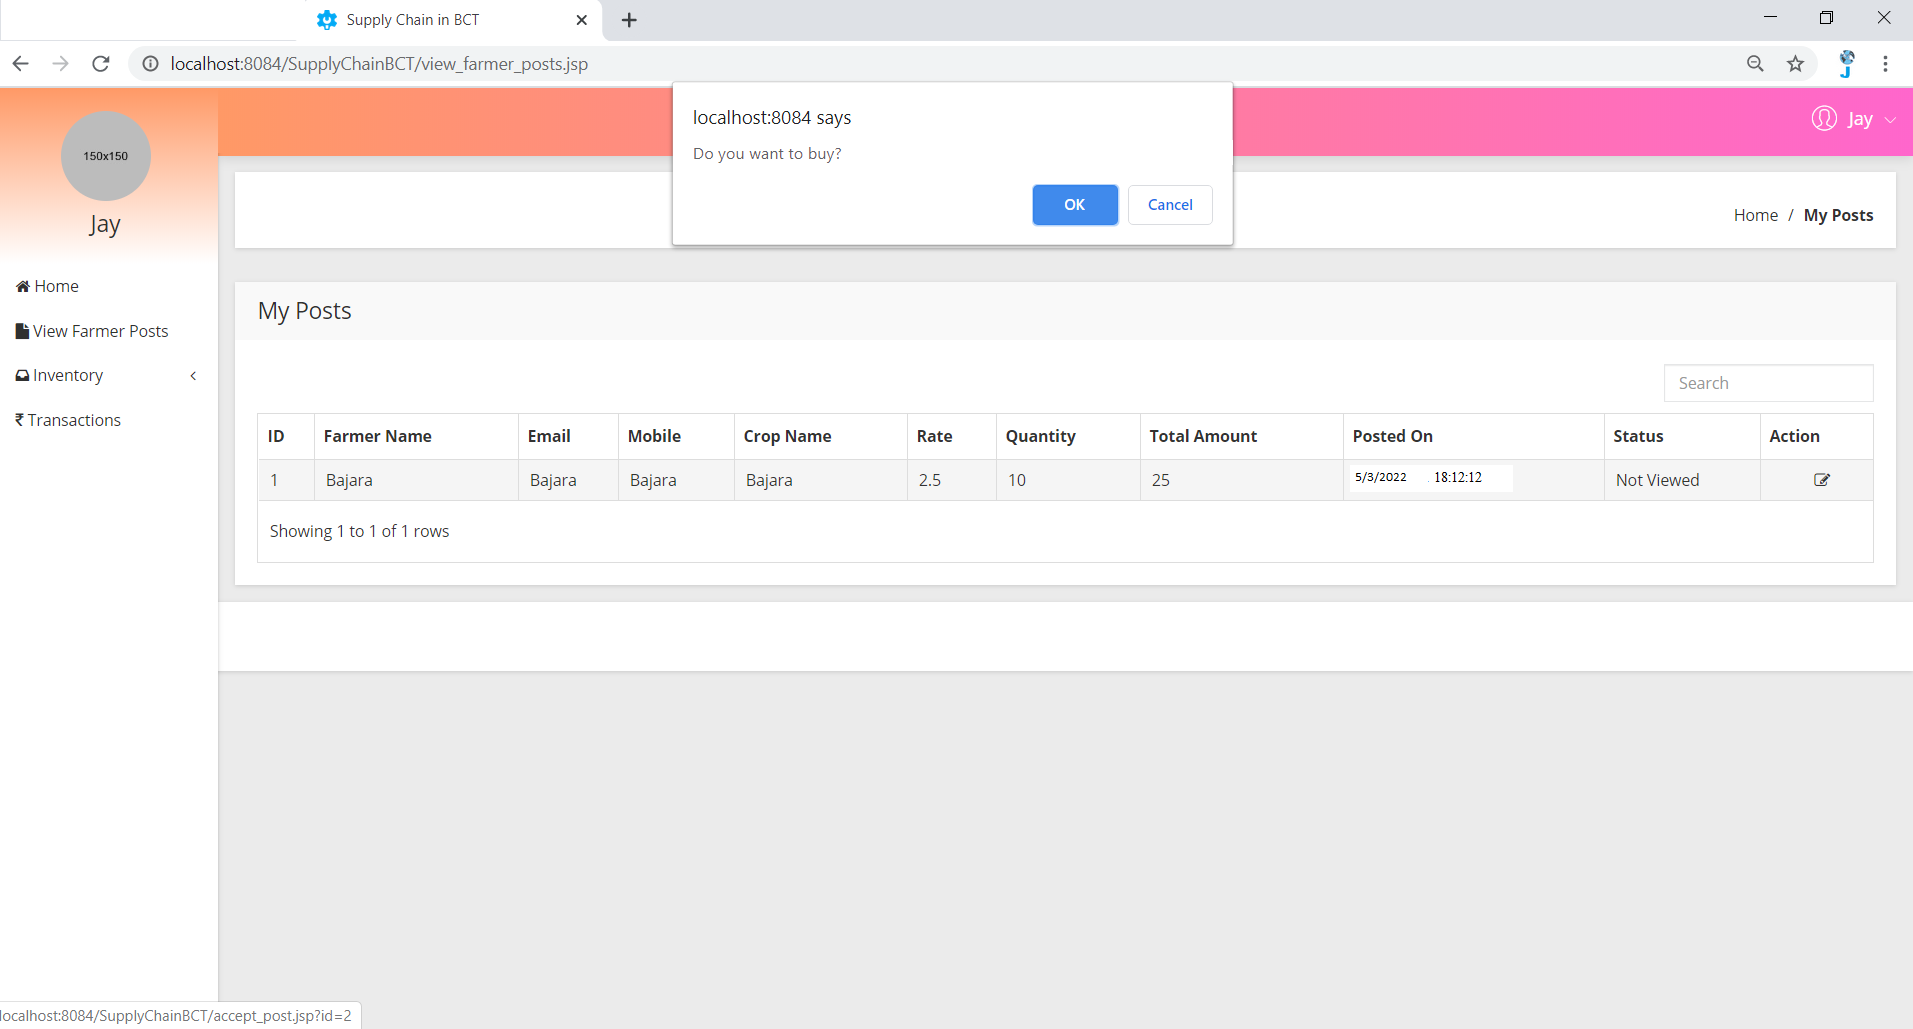
\includegraphics[scale=0.30]{10BuyFamerProduct}}
		\caption{Buy Famer Product}
		\label{fig:Buy Famer Product}
	\end{figure}
\end{center}

\begin{center}
	\begin{figure}[!htbp]
		\centering
		\fbox{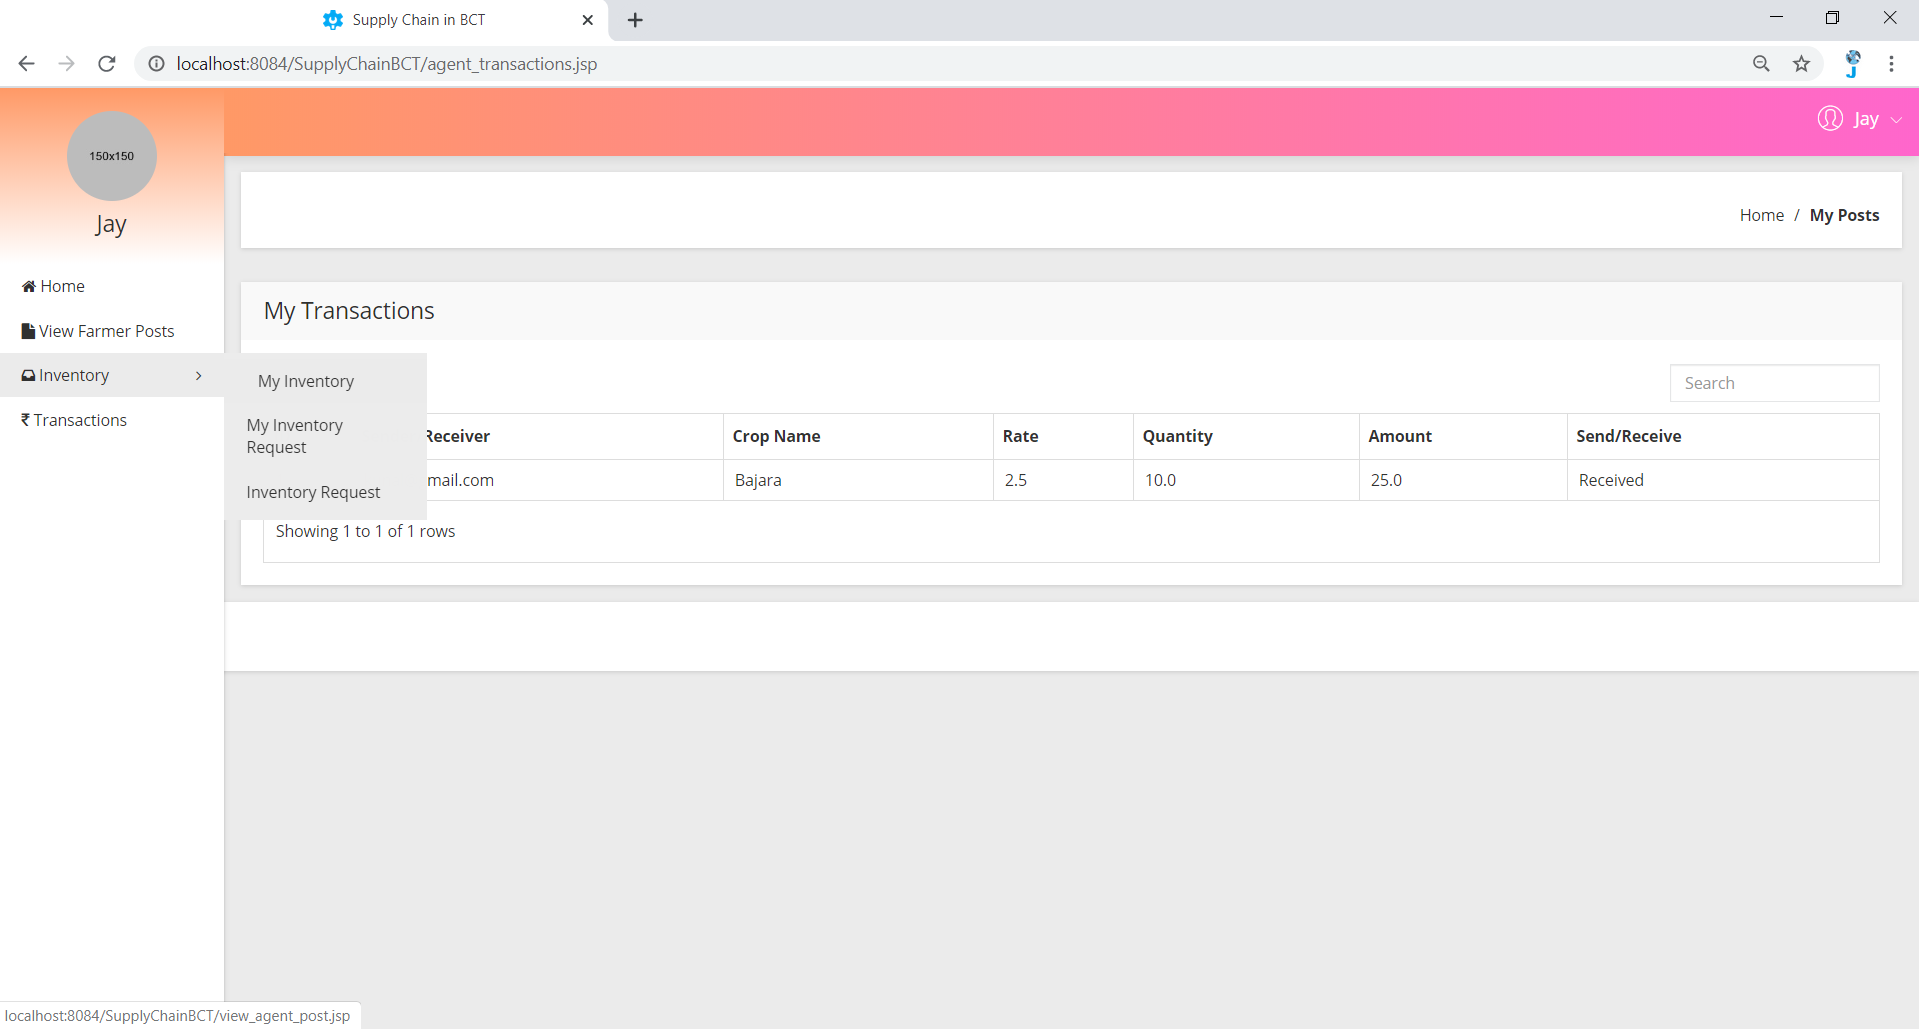
\includegraphics[scale=0.30]{12AgentInventory}}
		\caption{Agent Inventory}
		\label{fig:Agent Inventory}
	\end{figure}
\end{center}
\newpage


\chapter{Conclusion}:

Thus we are have implemented a prototype web based software application in Java for application of BCT in supply chain management . We have implemented block chain features such as:
1.	Decentralization
2.	Visual Cryptography
3.	Hash Algorithm
4.	Encrypted Database.
Thus it is possible to track agricultural supply chain and to give minimum price for agricultural products. 
\section{Future Scope}

In future we will try for sponsorship from government and will implement a project on large scale with some domain and hosting space online.

\section{Applications}

1.	Farmers\newline
2.	Government Organizations\newline
3.	Banking Sector.\newline




%-----------------------------------------------------------------------------------------------------------

%\section{Analysis Models: SDLC Model to be applied}
%\begin{itemize}
%\item \textbf{Waterfall Model}\\
%The Waterfall Model was first Process Model to be introduced. It is also referred to as a linear-sequential life cycle model. It is very simple to understand and use. In a waterfall model, each phase must be completed fully before the next phase can begin. This type of model is basically used for the for the project which is small and there are no uncertain requirements. At the end of each phase, a review takes place to determine if the project is on the right path and whether or not to continue or discard the project. In this model the testing starts only after the development is complete. In waterfall model phases do not overlap.
%\begin{center}
%	\begin{figure}[!htbp]
%		\centering
%		\fbox{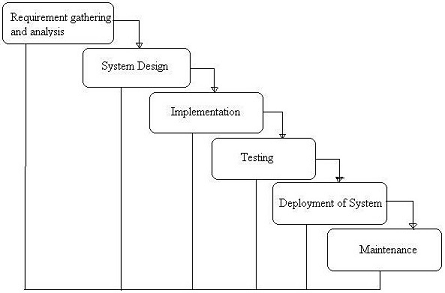
\includegraphics[scale=1]{wt}}
%	  \caption{Waterfall Model}
%	  \label{fig:Waterfall Model}
%	\end{figure}
%\end{center}
%\newpage
%\item \textbf{Applications}
%\begin{enumerate}
%\item This model is simple and easy to understand and use.
%\item It is easy to manage due to the rigidity of the model,each phase has specific deliverables and a review process.
%\item  In this model phases are processed and completed one at a time. Phases do not overlap.
%\item Waterfall model works well for smaller projects where requirements are very well understood.
%\end{enumerate}
%\end{itemize}
%\newpage
%\section{System Implementation Plan}
%\begin{center}
%	\begin{figure}[!htbp]
%		\centering
%		\fbox{\includegraphics[width=15cm, height=10cm]{plan}}
%	  \caption{Project Plan}
%	  \label{fig:Project Plan}
%	\end{figure}
%\end{center} 


%--------------------------------------------------
\chapter{REFERENCES}
\begin{enumerate}
\item L. Guo, C. Zhang, J. Sun, Y. Fang. “A privacy-preserving attribute based authentication System for Mobile Health Networks", IEEE Transactions on Mobile Computing, 2014.

\item A. Abbas, S. Khan, “ A review on the state-of-the-art privacy preserving approaches in e-health clouds", IEEE Journal of Biomedical Health Informatics, 2014.

\item J. Yang, J. Li, Y. Niu, “ A hybrid solution for privacy preserving medi-cal data sharing in the cloud environment ”, Future Generation Computer Systems, 2015.

\item V. Goyal, O. Pandey, A. Sahai, B. Waters, “ Attribute-based encryption for fine-grained access control of encrypted data ”, Proc. 13thm ACM Conf. Computer and Comm. Security (CCS06), 2006.

\item R. Ostrovsky, A. Sahai, B.Waters, “ Attribute-based encryption with non-monotonic access structures ”, in: Proceedings of the 14th ACM Confer-ence on Computer and Communications Security, ACM, 2007.

\item J. Han, W. Susilo, Y. Mu. “ Improving privacy and security in decentralized cipher text-policy attribute-based encryption ”, IEEE Transactions on on Information Forensics and Security, 2015.

\item M. Li, S. Yu, Y. Zheng, K. Ren, W. Lou, “ Scalable and secure sharing of personal health records in cloud computing using attribute based encryp-tion ”, IEEE transactions on parallel and distributed systems, 2013.

\item M. Green, S. Hohenberger, B. Waters, “ Outsourcing the decryption of ABE ciphertexts ”, in Proc. USENIX Security Symp., San Francisco, CA, USA, 2011.

\item J. Lai, R. H. Deng, C. Guan, J. Weng, “Attribute-based encryption with verifiable outsourced decryption ”, IEEE Trans. Inf. Forensics Security, Aug. 2013.

\item B. Qin, R. H. Deng, S. Liu, S. Ma, “Attribute-based encryption with efficient verifiable outsourced decryption ”, IEEE Trans. Inf. Forensics Security, JULY. 2015.

\end{enumerate}

\begin{appendices}
\chapter{}
\begin{itemize}

\item Definitions: P, NP, NP-Hard, NP-Complete Problems:

\item P Class of problems: Solutions to P class of problems have  deterministic algorithms running  in polynomial.
\item NP Class of problems: Solutions to NP class of problems have non-deterministic algorithms running in polynomial.
\item NP-Hard class of problems: A problem is in NP-Hard class if an already proved NP-Hard problem reduces to it.
\item NP-Complete class of problems: A problem is NP-Complete if it is NP-Hard and it is NP  (i.e. there exists a non-deterministic algorithm running in polynomial time which solves it).

Therefore, our system is NP-Complete. Hence it Is Feasible.

\end{itemize}

\begin{center}
	\begin{figure}[!htbp]
		\centering
		\fbox{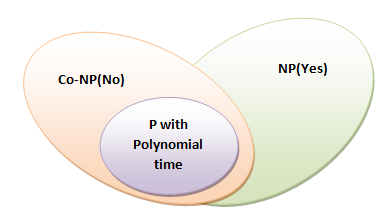
\includegraphics[scale=0.80]{np1}}
   	    \caption{NP Problem}
	    \label{fig:NP Problem}
	\end{figure}
\end{center}

\begin{itemize}




\item What is NP?
•	"NP" means "we can solve it in polynomial time if we can break the normal rules of step-by-step computing".
\item What is NP-Complete?
•	Since this amazing "N" computer can also do anything a normal computer can, we know that "P" problems are also in "NP".
•	So, the easy problems are in "P" (and "NP"), but the really hard ones are *only* in "NP", and they are called "NP-complete".
•	It is like saying there are things that People can do ("P"), there are things that Super People can do ("SP"), and there are things *only* Super People can do ("SP-complete").
\item NP-Complete:
We have use Bloom filtering for detection of packet drop attack whether it is drop by itself or by hacker.  
Hence the ‘P’ is NP-Complete in this case.


\end{itemize}


\begin{center}
	\begin{figure}[!htbp]
		\centering
		\fbox{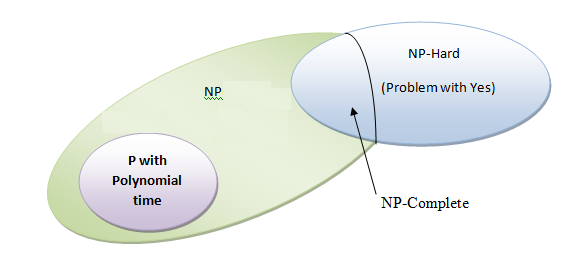
\includegraphics[scale=0.80]{np2}}
   	    \caption{NP Problem Complete}
	    \label{fig:NP Problem Complete}
	\end{figure}
\end{center}

\end{appendices}

\end{document}
%-------------------------------------------------------------------
